\documentclass[11pt,oneside]{book}

\usepackage[a4paper,margin=27mm,headheight=15pt]{geometry}
\usepackage[T1]{fontenc}
\usepackage[utf8]{inputenc}
\IfFileExists{libertinus.sty}{\usepackage{libertinus}}{\usepackage{lmodern}}
\usepackage{microtype}
\usepackage{amsmath,amssymb,amsthm,mathtools,mathrsfs,bm}
% Canonical mathematical notation for active FabiusFunction LaTeX documents.
%
% This file is intentionally a plain TeX input rather than a LaTeX package.
% Every standalone document loads it by an explicit path relative to that
% document's directory; included fragments inherit the definitions from their
% root document.  Keep this file independent of document layout and metadata.
%
% Contract:
%   * one command has one mathematical meaning throughout the active corpus;
%   * names encode semantic roles rather than a document-local choice of letter;
%   * visually similar but differently normalized objects have different print;
%   * every command below is defined normatively in the notation catalogue.
%
% The active corpus excludes docs/archive/.  Historical sources may retain
% their original notation only inside an explicitly labelled quotation.

\makeatletter
\@ifundefined{mathbb}{%
  \PackageError{fabius-notation}{The amssymb package must be loaded first}%
    {Load amsmath and amssymb before inputting fabius-notation.tex.}%
}{}
\@ifundefined{operatorname}{%
  \PackageError{fabius-notation}{The amsmath package must be loaded first}%
    {Load amsmath before inputting fabius-notation.tex.}%
}{}
\makeatother

% Version stamp used by the catalogue and by static audits.
\newcommand{\FabiusNotationVersion}{2026-08-31}

% Number systems.  NaturalNumbers is explicitly the nonnegative convention.
\newcommand{\NaturalNumbers}{\mathbb{N}_{0}}
\newcommand{\PositiveIntegers}{\mathbb{N}_{>0}}
\newcommand{\IntegerNumbers}{\mathbb{Z}}
\newcommand{\RationalNumbers}{\mathbb{Q}}
\newcommand{\RealNumbers}{\mathbb{R}}
\newcommand{\ComplexNumbers}{\mathbb{C}}
\newcommand{\ExtendedRealNumbers}{\overline{\mathbb{R}}}

% The three principal Fabius--Rvachev functions.  Subscripts are deliberate:
% a bare F and a calligraphic F have several unrelated uses in the corpus.
\newcommand{\FabiusBounded}{F_{\mathrm{bd}}}
\newcommand{\FabiusGlobal}{F_{\mathrm{gl}}}
\newcommand{\FabiusQuantile}{Q_{F}}
\newcommand{\FabiusClampedQuantile}{Q_{F,\mathrm{cl}}}
\newcommand{\RvachevUp}{\operatorname{up}}

% Constants, elementary operators, and delimiters.
\newcommand{\EulerE}{\mathrm{e}}
\newcommand{\ImaginaryUnit}{\mathrm{i}}
\newcommand{\Differential}{\mathop{}\!\mathrm{d}}
\newcommand{\AbsoluteValue}[1]{\left\lvert #1\right\rvert}
\newcommand{\Norm}[1]{\left\lVert #1\right\rVert}
\newcommand{\Floor}[1]{\left\lfloor #1\right\rfloor}
\newcommand{\Ceiling}[1]{\left\lceil #1\right\rceil}
\newcommand{\FractionalPart}[1]{\left\{#1\right\}}
\newcommand{\PositivePart}[1]{\left(#1\right)_{+}}
\newcommand{\IndicatorOf}[1]{\mathbf{1}_{#1}}
\newcommand{\SetOf}[1]{\left\{#1\right\}}
\newcommand{\InnerProduct}[1]{\left\langle #1\right\rangle}
\newcommand{\CardinalityOf}[1]{\left\lvert #1\right\rvert}
\newcommand{\DefinitionEquals}{\mathrel{\coloneqq}}
\newcommand{\Sign}{\operatorname{sgn}}
\newcommand{\IdentityOperator}{\operatorname{id}}
\newcommand{\SpanOperator}{\operatorname{span}}
\newcommand{\TraceOperator}{\operatorname{tr}}
\newcommand{\RankOperator}{\operatorname{rank}}
\newcommand{\DiagonalOperator}{\operatorname{diag}}
\newcommand{\ResidueOperator}{\operatorname*{Res}}
\newcommand{\LeastCommonMultiple}{\operatorname{lcm}}
\newcommand{\OrderOperator}{\operatorname{ord}}
\newcommand{\PrincipalLogarithm}{\operatorname{Log}}
\newcommand{\FallingFactorial}[2]{\left(#1\right)^{\underline{#2}}}
\newcommand{\RisingFactorial}[2]{\left(#1\right)^{\overline{#2}}}

% Support, topology, convolution, and metric notation.
\newcommand{\SupportOperator}{\operatorname{supp}}
\newcommand{\SupportOf}[1]{\SupportOperator\!\left(#1\right)}
\newcommand{\TopologicalSupportOf}[1]{\operatorname{tsupp}\!\left(#1\right)}
\newcommand{\Convolution}{\mathbin{*}}
\newcommand{\MetricDistance}{\operatorname{dist}}
\newcommand{\TotalVariationDistance}{d_{\mathrm{TV}}}

% Probability.  Equality and convergence in law are not metric distance.
\newcommand{\Probability}{\mathbb{P}}
\newcommand{\Expectation}{\mathbb{E}}
\newcommand{\Variance}{\operatorname{Var}}
\newcommand{\Covariance}{\operatorname{Cov}}
\newcommand{\LawOperator}{\operatorname{Law}}
\newcommand{\LawOf}[1]{\LawOperator\!\left(#1\right)}
\newcommand{\EqualInLaw}{\mathrel{\overset{\mathrm{law}}{=}}}
\newcommand{\ConvergesInLaw}{\mathrel{\xrightarrow{\mathrm{law}}}}

% Fourier and integral transforms.  The printed labels expose normalization.
% FourierTwoPi uses exp(-2*pi*i*x*xi); FourierAngular uses exp(-i*x*omega).
\newcommand{\FourierTwoPi}[1]{\widehat{#1}_{\,2\pi}}
\newcommand{\FourierAngular}[1]{\widehat{#1}_{\,\mathrm{ang}}}
\newcommand{\LaplaceTransformSymbol}{\mathcal{L}}
\newcommand{\MellinTransformSymbol}{\mathcal{M}}
\newcommand{\LaplaceTransformOf}[1]{\LaplaceTransformSymbol\!\left[#1\right]}
\newcommand{\MellinTransformOf}[1]{\MellinTransformSymbol\!\left[#1\right]}
\newcommand{\MomentGeneratingFunction}[1]{M_{#1}}
\newcommand{\CharacteristicFunction}[1]{\varphi_{#1}}

% The two standard sinc functions must never share one symbol.
\newcommand{\SincRad}{\operatorname{sinc}_{\mathrm{rad}}}
\newcommand{\SincPi}{\operatorname{sinc}_{\pi}}

% Binary arithmetic and Thue--Morse notation.
\newcommand{\BinaryDigitSum}{\operatorname{wt}_{2}}
\newcommand{\ThueMorseSignSymbol}{\varepsilon}
\newcommand{\ThueMorseSign}[1]{\varepsilon_{#1}}
\newcommand{\PadicValuation}[1]{\nu_{#1}}
\newcommand{\TwoAdicValuation}{\nu_{2}}

% q-series notation.  Every base is an explicit argument.
\newcommand{\QPochhammer}[3]{\left(#1;#2\right)_{#3}}
\newcommand{\GaussianBinomial}[3]{%
  \genfrac{[}{]}{0pt}{}{#1}{#2}_{#3}%
}
\newcommand{\QInteger}[2]{\left[#1\right]_{#2}}

% Named special functions.
\newcommand{\Polylogarithm}{\operatorname{Li}}
\newcommand{\LambertW}{W}
\newcommand{\GammaFunction}{\Gamma}
\newcommand{\RiemannZeta}{\zeta}

% Asymptotics.  BigO and LittleO are operator tokens for existing formula
% grammar; prefer the At forms so that the limiting regime is printed.
\newcommand{\BigO}{\mathcal{O}}
\newcommand{\LittleO}{o}
\newcommand{\BigOAt}[2]{\mathcal{O}_{#2}\!\left(#1\right)}
\newcommand{\LittleOAt}[2]{o_{#2}\!\left(#1\right)}

\usepackage{booktabs,longtable,tabularx,array}
\usepackage{graphicx}
\usepackage{xcolor}
\usepackage{enumitem}
\usepackage{fancyhdr}
\usepackage{titlesec}
\usepackage{xurl}
\usepackage{listings}
\usepackage{hyperref}
\usepackage[nameinlink,noabbrev,capitalise]{cleveref}

\definecolor{linkblue}{RGB}{30,76,128}
\definecolor{deepgreen}{RGB}{34,103,75}
\definecolor{deepred}{RGB}{142,48,48}
\definecolor{shadegray}{RGB}{246,247,249}
\definecolor{rulegray}{RGB}{190,198,205}

\hypersetup{
  colorlinks=true,
  linkcolor=linkblue,
  citecolor=deepgreen,
  urlcolor=linkblue,
  pdftitle={Geometric-Comb Interpolation, Gaussian Pascal Transforms, and the Fabius--Rvachev Boundary Layer},
  pdfauthor={OpenAI GPT-5.6 Pro},
  pdfsubject={Lagrange and Newton interpolation on geometric combs; q-Pochhammer and Gaussian-binomial structure; Fabius and Rvachev applications},
  pdfkeywords={geometric interpolation, Newton interpolation, Lagrange interpolation, q-Pochhammer, Gaussian binomial, Fabius function, Rvachev up-function, Lebesgue constant, q-calculus}
}

\pagestyle{fancy}
\fancyhf{}
\fancyhead[L]{\small Geometric-comb interpolation}
\fancyhead[R]{\small\nouppercase{\leftmark}}
\fancyfoot[C]{\thepage}
\renewcommand{\headrulewidth}{0.4pt}

\titleformat{\chapter}[display]
  {\normalfont\huge\bfseries\color{linkblue}}
  {\filleft\Large\chaptertitlename\ \thechapter}
  {0.7ex}{\titlerule[0.6pt]\vspace{1ex}\filright}
\titleformat{\section}{\Large\bfseries\color{linkblue}}{\thesection}{0.72em}{}
\titleformat{\subsection}{\large\bfseries\color{deepgreen}}{\thesubsection}{0.65em}{}
\titleformat{\subsubsection}{\normalsize\bfseries}{\thesubsubsection}{0.58em}{}

\setcounter{tocdepth}{2}
\setcounter{secnumdepth}{3}
\numberwithin{equation}{chapter}
\allowdisplaybreaks[3]
\setlength{\emergencystretch}{3em}
\setlist[itemize]{leftmargin=2em,itemsep=0.25em,topsep=0.45em}
\setlist[enumerate]{leftmargin=2.3em,itemsep=0.25em,topsep=0.45em}
\graphicspath{{figures/}}

\lstset{
  basicstyle=\ttfamily\small,
  columns=fullflexible,
  keepspaces=true,
  frame=single,
  rulecolor=\color{rulegray},
  backgroundcolor=\color{shadegray},
  breaklines=true,
  showstringspaces=false,
  tabsize=4
}

\newtheorem{theorem}{Theorem}[chapter]
\newtheorem{lemma}[theorem]{Lemma}
\newtheorem{proposition}[theorem]{Proposition}
\newtheorem{corollary}[theorem]{Corollary}
\newtheorem{identity}[theorem]{Identity}
\theoremstyle{definition}
\newtheorem{definition}[theorem]{Definition}
\newtheorem{example}[theorem]{Example}
\newtheorem{algorithm}[theorem]{Algorithm}
\newtheorem{conjecture}[theorem]{Conjecture}
\newtheorem{problem}[theorem]{Research problem}
\theoremstyle{remark}
\newtheorem{remark}[theorem]{Remark}
\newtheorem{observation}[theorem]{Numerical observation}

\newcommand{\Nzero}{\mathbb N_0}
\newcommand{\halfbinom}[2]{\GaussianBinomial{#1}{#2}{1/2}}
\newcommand{\twobinom}[2]{\GaussianBinomial{#1}{#2}{2}}
\newcommand{\App}{\mathcal A}
\newcommand{\Interp}{\mathcal I}
\newcommand{\Leb}{\Lambda}
\newcommand{\MGF}{\mathcal M}
\newcommand{\PiN}{\Pi}
\DeclareMathOperator{\ord}{ord}

\newenvironment{resultbox}
{\par\medskip\noindent\begin{center}\begin{minipage}{0.94\textwidth}\hrule\medskip}
{\medskip\hrule\end{minipage}\end{center}\medskip}

\title{\bfseries Geometric-Comb Interpolation, Gaussian Pascal Transforms,\\[0.25em]
       and the Fabius--Rvachev Boundary Layer\\[0.6em]
       \Large Lagrange/Newton theory on $c q^{\Nzero}$, exact $q$-residuals,\\
       a sharp stability dichotomy, and dyadic atomic-function applications}
\author{OpenAI GPT-5.6 Pro\\[0.4em]
\small Research report prepared for Vladimir Reshetnikov}
\date{30 August 2026\\[0.2em]
\small ProveIt repository snapshot \texttt{e5175d5eb78d66f4e31db3bc506541b9bae12c57}}

\begin{document}
\frontmatter
\hypersetup{pageanchor=false}
\maketitle
\hypersetup{pageanchor=true}
\pagenumbering{roman}

\chapter*{Abstract}
\addcontentsline{toc}{chapter}{Abstract}
\begin{quote}
Let $0<q<1$, $c>0$, and consider the finite geometric comb
$\{c,cq,\ldots,cq^n\}$, together with its accumulation point $0$.
At these nodes, ordinary Newton interpolation is already a piece of
$q$-calculus: its basis polynomials are the shifted factorials
\[
 N_k(x;c,q)=\prod_{r=0}^{k-1}(x-cq^r)
 =(-c)^kq^{\binom k2}(x/c;q^{-1})_k,
\]
and its divided differences are normalized iterates of the Jackson
$q$-derivative.  This report develops that observation into a systematic
interpolation theory.  It proves explicit Lagrange and barycentric formulas,
a Gaussian-Pascal change of basis between monomials and geometric Newton
polynomials, an exact complete-homogeneous residual formula for every
monomial and analytic function, a convergent infinite Newton expansion for
functions analytic across the accumulation point, and an exact
Newton--Jackson quadrature identity.

The stability theory has a particularly sharp two-sided answer.  Extrapolation
to the accumulation point is uniformly bounded:
\[
 \Leb_n(0)=\frac{(-q;q)_n}{(q;q)_n}
 \longrightarrow\frac{(-q;q)_\infty}{(q;q)_\infty}.
\]
In contrast, the global Lebesgue constant on $[0,c]$ is
superexponential.  A boundary-layer analysis proved here gives
\[
 \max_{0\le x\le c}\Leb_n(x)
 \sim \frac{2(-q;q)_\infty}{\EulerE}
       \frac{q^{-\binom n2}}{n},
 \qquad
 \frac{x_n^*}{c}=1-\frac1n+o(n^{-1}).
\]
Thus the same comb is a stable extrapolation device at the end where it
accumulates and a violently ill-conditioned global interpolation device in
the persistent outer gap.

For $q=1/2$, the nodes are precisely the inverse-dyadic scales naturally
selected by the Fabius function.  Writing $a_j=\Expectation X^j/j!$ for the Fabius
moment coefficients, the geometric Newton coefficients become the exact
base-$2$ Gaussian transform
\[
 [F;1,2^{-1},\ldots,2^{-k}]
 =\frac1{(1/2;1/2)_k}
   \sum_{j=0}^k(-1)^j\twobinom{k}{j}a_j.
\]
The report derives a finite Gaussian-cardinal formula for the entire
interpolant, a $q$-Borel-type generating function for its boundary residues,
and superexponential bounds proving recovery of every fixed flat endpoint
jet even though $F$ is nonanalytic there.  Simultaneously, exact rational
experiments show rapid divergence inside the gap $(1/2,1)$ and motivate a
sharp saddle-point conjecture.  Reflecting $x=1-t$ transfers the results to
the Rvachev function $\RvachevUp(t)=F(1-|t|)$ on its boundary comb
$t_j=1-2^{-j}$.  Finally, exact polynomial reproduction by translates of
$\RvachevUp$ is composed with the geometric Lagrange operator, producing a finite
Gaussian--Appell decoder and a closed interpolation/synthesis loop.

Statements labeled theorem, proposition, lemma, or corollary are proved.
Unproved asymptotic claims are explicitly labeled conjectures.  The bundled
Python program uses exact rational arithmetic wherever possible and
logarithmic floating-point arithmetic only for the enormous Lebesgue
constants.
\end{quote}

\chapter*{Executive summary of the main formulas}
\addcontentsline{toc}{chapter}{Executive summary of the main formulas}

The geometric comb is more than a convenient nonuniform grid.  It is the
node geometry for which the Newton product, divided-difference operator,
Gaussian coefficients, complete homogeneous functions, and Jackson
integration all close under explicit finite formulae.

\begin{resultbox}
For $x_j=cq^j$ and $N_k(x)=\prod_{r<k}(x-x_r)$,
\begin{align*}
 N_k(x)&=(-c)^kq^{\binom k2}(x/c;q^{-1})_k,\\
 [f;x_0,\ldots,x_k]
 &=\frac{D_q^kf(c)}{[k]_q!}\\
 &=c^{-k}\sum_{j=0}^k
 \frac{(-1)^jq^{-jk+\binom{j+1}{2}}}
 {(q;q)_j(q;q)_{k-j}}f(cq^j),\\
 x^m&=\sum_{k=0}^m c^{m-k}\GaussianBinomial{m}{k}{q}N_k(x),\\
 N_k(x)&=\sum_{m=0}^k(-1)^{k-m}c^{k-m}
 q^{\binom{k-m}{2}}\GaussianBinomial{k}{m}{q}x^m.
\end{align*}
The last two displays are mutually inverse Gaussian-Pascal transforms.
\end{resultbox}

\begin{resultbox}
For the degree-$n$ interpolant $\Interp_nf$,
\[
 x^{n+1+r}-\Interp_n(x^{n+1+r})
 =N_{n+1}(x)h_r(x,c,cq,\ldots,cq^n),
\]
and
\[
 h_r(x,c,cq,\ldots,cq^n)
 =\sum_{s=0}^r x^s c^{r-s}\GaussianBinomial{n+r-s}{n}{q}.
\]
This is the exact all-orders interpolation residual; the usual remainder
with an unspecified intermediate derivative is replaced by an explicit
$q$-polynomial.
\end{resultbox}

\begin{resultbox}
For the Fabius function and $q=1/2$,
\begin{align*}
 F(2^{-j})&=2^{-\binom j2}a_j,\\
 \Interp_nF(x)
 &=\frac{\prod_{r=0}^n(x-2^{-r})}{(1/2;1/2)_n}
   \sum_{j=0}^n
   \frac{(-1)^j\twobinom{n}{j}a_j}{x-2^{-j}},\\
 \sum_{n\ge0}(\Interp_nF)(0)z^n
 &=(z/2;1/2)_\infty
   \sum_{j\ge0}\frac{2^{-\binom j2}a_j}{(1/2;1/2)_j}z^j.
\end{align*}
At $x=0$ the residues decay at least like
$2^{-\Floor{n^2/4}}$ up to a fixed factor; at $x=3/4$ they grow, according
to exact rational data, on the conjectural scale
$2^{n^2/4}n^{-n/2}\EulerE^{O(n)}$.
\end{resultbox}

\tableofcontents
\mainmatter

\part{Algebra of the geometric comb}

\chapter{Scope, provenance, and normalization}
\label{chap:scope}

\section{Relation to the source monograph and neighboring reports}

The starting point is the chapter on negative upper indices and geometric
Newton interpolation in
\path{q_pochhammer_q_binomial_monograph.tex}.  That chapter already records
the basic divided-difference formula on $1,q,\ldots,q^n$.  The present report
expands that seed in four directions:

\begin{enumerate}
\item it develops the full change-of-basis and residual algebra, rather than
      treating geometric interpolation as an isolated application;
\item it separates local convergence near the accumulation point from global
      stability on the convex hull and proves sharp asymptotics for both;
\item it specializes the transforms to the inverse-dyadic Fabius data and
      obtains exact boundary-residue and endpoint-jet estimates;
\item it composes the geometric interpolant with the existing Rvachev
      polynomial-synthesis operator, thereby connecting $q$-Pochhammer
      coordinates to finite dictionaries of compactly supported atomic
      functions.
\end{enumerate}

The uniform dyadic-comb report is used only for comparison: its nodes
$j/2^m$ fill $[0,1]$ but suffer the familiar global high-degree instability.
The geometric comb $2^{-j}$ has a different pathology: it samples one
boundary on all binary scales, but it leaves a fixed gap $(1/2,1)$.  The
Rvachev--Lagrange loop report supplies the exact inverse-moment Appell
synthesis of polynomials by translates of $\RvachevUp$.  Results imported from those
reports are identified when used; the new derivations are proved here.

All novelty statements are relative to the audited repository snapshot in
the title, not claims of unrestricted world priority.  Classical background
on $q$-series and $q$-calculus is available in
\cite{Andrews1986,GasperRahman2004,KacCheung2002,DLMF17}; the $q$-Newton
viewpoint is particularly explicit in \cite{Kupershmidt2000}.  Barycentric
interpolation and its numerical evaluation are treated in
\cite{BerrutTrefethen2004,Higham2004}.

\section{The affine geometric comb}

\begin{definition}[Affine geometric comb]
Let $\alpha,\beta,q\in\ComplexNumbers$ with $\beta\ne0$.  The degree-$n$ affine geometric
comb is
\[
 \mathcal G_n(\alpha,\beta;q)
 :=\{\alpha+\beta q^j:0\le j\le n\}.
\]
When $|q|<1$, its infinite continuation accumulates at $\alpha$.  The
multiplicative normalization is $\alpha=0$, $\beta=c$; the reflected
boundary normalization used for $\RvachevUp$ is $\alpha=1$, $\beta=-1$.
\end{definition}

Finite interpolation requires distinct nodes, equivalently
$q^d\ne1$ for $1\le d\le n$.  Most algebraic formulae remain valid over an
arbitrary field under that hypothesis.  The convergence and Lebesgue theory
will assume
\begin{equation}
 0<q<1,
 \qquad c>0,
 \qquad x_j=cq^j.
 \label{eq:real-normalization}
\end{equation}
The affine case is recovered by $z=(x-\alpha)/\beta$.

\begin{proposition}[Affine covariance]
Let $P$ interpolate $f$ on $\mathcal G_n(\alpha,\beta;q)$ and set
$g(z)=f(\alpha+\beta z)$.  If $Q$ interpolates $g$ on
$1,q,\ldots,q^n$, then
\[
 P(x)=Q\!\left(\frac{x-\alpha}{\beta}\right).
\]
The Lagrange cardinals transform by the same substitution, and the Lebesgue
function is invariant under real affine changes that map the interpolation
interval bijectively to itself.
\end{proposition}

\begin{proof}
Both sides are polynomials of degree at most $n$ and agree at all $n+1$
nodes.  The cardinal and Lebesgue assertions follow immediately.
\end{proof}

Thus $c$ is retained in algebraic formulae to expose homogeneity, but it can
be set to $1$ in all conditioning arguments.

\section{Notation for \texorpdfstring{$q$}{q}-analogues}

For $k\in\Nzero$,
\begin{align}
 (a;q)_k&:=\prod_{r=0}^{k-1}(1-aq^r),
 & (a;q)_0&:=1,\\
 [k]_q&:=\frac{1-q^k}{1-q},
 & [k]_q!&:=\prod_{r=1}^k[r]_q=\frac{(q;q)_k}{(1-q)^k},\\
 \GaussianBinomial{n}{k}{q}&:=\frac{(q;q)_n}{(q;q)_k(q;q)_{n-k}}
 &&(0\le k\le n).
\end{align}
The Gaussian coefficient is a polynomial in $q$; quotient notation is used
only where the displayed denominators are nonzero.  Reciprocity reads
\begin{equation}
 \GaussianBinomial{n}{k}{q^{-1}}=q^{-k(n-k)}\GaussianBinomial{n}{k}{q}.
 \label{eq:q-reciprocity}
\end{equation}
The complete homogeneous symmetric polynomial is characterized by
\begin{equation}
 \prod_{j=0}^m\frac1{1-y_jt}
 =\sum_{r\ge0}h_r(y_0,\ldots,y_m)t^r.
 \label{eq:h-generating}
\end{equation}
Its geometric principal specialization is
\begin{equation}
 h_r(c,cq,\ldots,cq^m)=c^r\GaussianBinomial{m+r}{m}{q}.
 \label{eq:h-principal}
\end{equation}
This simple identity is the source of almost every Gaussian coefficient in
the residual formulae below.

\chapter{Newton interpolation as \texorpdfstring{$q$}{q}-Taylor calculus}
\label{chap:q-newton}

\section{The \texorpdfstring{$q$}{q}-Pochhammer Newton basis}

\begin{definition}[Geometric Newton polynomial]
For $k\ge0$, define
\begin{equation}
 N_k(x;c,q):=\prod_{r=0}^{k-1}(x-cq^r),
 \qquad N_0:=1.
 \label{eq:newton-basis}
\end{equation}
\end{definition}

The factor locations are exactly the first $k$ nodes of the comb.  Pulling
out $-cq^r$ from each factor gives the fundamental identification
\begin{equation}
 \boxed{
 N_k(x;c,q)=(-c)^kq^{\binom k2}(x/c;q^{-1})_k.}
 \label{eq:newton-pochhammer}
\end{equation}
Thus the finite $q$-Pochhammer symbol is not merely analogous to a Newton
basis: on a geometric grid it \emph{is} the Newton basis, up to its monic
normalization.

Let
\begin{equation}
 (D_qf)(x):=\frac{f(x)-f(qx)}{(1-q)x},
 \qquad x\ne0,
 \label{eq:Dq}
\end{equation}
with the removable value at $0$ used when it exists.  The usual $q$-Leibniz
rule gives
\begin{equation}
 D_qN_k(x;c,q)=[k]_qN_{k-1}(x;c,q).
 \label{eq:Dq-newton}
\end{equation}
A direct proof follows by writing $N_k=(x-c)_{q}^{k}$ in the standard
$q$-falling-power notation.  The next theorem supplies the exact data-side
operator and fixes every power of $q$.

\begin{theorem}[Iterated Jackson difference and geometric divided difference]
\label{thm:Dq-divided-difference}
Let $E_qf(x)=f(qx)$.  For every $k\ge0$,
\begin{align}
 D_q^k
 &=\frac{x^{-k}}{(1-q)^k}(E_q;q^{-1})_k,
 \label{eq:Dq-operator-factor}\\
 D_q^kf(x)
 &=\frac{x^{-k}}{(1-q)^k}
   \sum_{j=0}^k(-1)^j
   q^{-jk+\binom{j+1}{2}}\GaussianBinomial{k}{j}{q}f(q^jx).
 \label{eq:Dq-explicit}
\end{align}
Consequently, for distinct nodes $c,cq,\ldots,cq^k$,
\begin{equation}
 \boxed{
 [f;c,cq,\ldots,cq^k]
 =\frac{D_q^kf(c)}{[k]_q!}
 =c^{-k}\sum_{j=0}^k
 \frac{(-1)^jq^{-jk+\binom{j+1}{2}}}
 {(q;q)_j(q;q)_{k-j}}f(cq^j).}
 \label{eq:geometric-divided-difference}
\end{equation}
\end{theorem}

\begin{proof}
As operators,
\[
 D_q=\frac{x^{-1}(1-E_q)}{1-q}.
\]
The commutation relation $E_qx^{-1}=q^{-1}x^{-1}E_q$ implies inductively
\[
 D_q^k=\frac{x^{-k}}{(1-q)^k}
       \prod_{r=0}^{k-1}(1-q^{-r}E_q),
\]
which is \eqref{eq:Dq-operator-factor}.  The finite $q$-binomial theorem at
base $q^{-1}$ gives
\[
 (E_q;q^{-1})_k
 =\sum_{j=0}^k(-1)^jq^{-\binom j2}
   \GaussianBinomial{k}{j}{q^{-1}}E_q^j.
\]
Using reciprocity \eqref{eq:q-reciprocity}, the exponent becomes
$-\binom j2-j(k-j)=-jk+\binom{j+1}{2}$, proving
\eqref{eq:Dq-explicit}.

It remains to identify the normalization.  Both functionals
$[f;c,cq,\ldots,cq^k]$ and $D_q^kf(c)/[k]_q!$ vanish on polynomials of degree
less than $k$.  Applied to $x^k$, the divided difference is $1$, while
$D_q^kx^k=[k]_q!$.  Equality follows on polynomials of degree at most $k$;
the explicit divided-difference formula, being a fixed linear combination of
point evaluations, then proves the equality for arbitrary data on the nodes.
Substituting $x=c$ in \eqref{eq:Dq-explicit} and using
$(1-q)^k[k]_q!=(q;q)_k$ gives the last expression.
\end{proof}

\begin{corollary}[$q$-Taylor form of the interpolant]
\label{cor:q-taylor-interpolant}
The polynomial of degree at most $n$ interpolating $f$ at
$c,cq,\ldots,cq^n$ is
\begin{equation}
 \boxed{
 (\Interp_nf)(x)=\sum_{k=0}^n
 \frac{D_q^kf(c)}{[k]_q!}N_k(x;c,q).}
 \label{eq:q-taylor-interpolant}
\end{equation}
\end{corollary}

\begin{proof}
This is the ordinary Newton interpolation formula with
\Cref{thm:Dq-divided-difference} substituted for each divided difference.
\end{proof}

\begin{remark}[Two meanings of ``$q$-Taylor'']
Formula \eqref{eq:q-taylor-interpolant} is simultaneously a polynomial
$q$-Taylor formula and a finite interpolation formula.  No limit process is
involved.  Infinite $q$-Taylor series require convergence hypotheses; those
are developed in \Cref{chap:infinite-newton}.
\end{remark}

\section{Triangular evaluation and the geometric Vandermonde determinant}

At a node $x=cq^j$, the basis evaluation is triangular:
\begin{equation}
 N_k(cq^j;c,q)=
 \begin{cases}
 (-c)^kq^{\binom k2}\dfrac{(q;q)_j}{(q;q)_{j-k}},&k\le j,\\[1.1ex]
 0,&k>j.
 \end{cases}
 \label{eq:newton-node-evaluation}
\end{equation}
This gives an $O(n^2)$ forward-substitution algorithm for the coefficients,
but it also exposes the determinant exactly.

\begin{theorem}[Geometric Vandermonde determinant]
\label{thm:geometric-vandermonde}
Let $V_n=(x_j^m)_{0\le j,m\le n}$ with $x_j=cq^j$, and put
$N=n(n+1)/2$.  Then
\begin{equation}
 \boxed{
 \det V_n=(-1)^N c^Nq^{\binom{n+1}{3}}
             \prod_{k=1}^n(q;q)_k.}
 \label{eq:geometric-vandermonde}
\end{equation}
\end{theorem}

\begin{proof}
The Vandermonde product is
\[
 \det V_n=\prod_{0\le r<s\le n}(cq^s-cq^r).
\]
For fixed $s$,
\[
 \prod_{r=0}^{s-1}(q^s-q^r)
 =(-1)^sq^{\binom s2}(q;q)_s.
\]
Multiplying over $s=1,\ldots,n$ gives the sign
$(-1)^{\sum s}=(-1)^N$, the power
$q^{\sum_s\binom s2}=q^{\binom{n+1}{3}}$, and the stated product.  There are
$N$ pairwise differences, giving $c^N$.
\end{proof}

The factor $q^{\binom{n+1}{3}}$ already signals severe monomial-Vandermonde
conditioning.  Newton coordinates remove the linear solve, but they do not
remove the intrinsic amplification of the interpolation operator.  That
amplification is measured exactly in \Cref{chap:stability}.

\section{Online extension of the comb}

Adding the new node $cq^{n+1}$ does not change any earlier Newton
coefficient.  Only
\begin{equation}
 \gamma_{n+1}
 =\frac{f(cq^{n+1})-\sum_{k=0}^n\gamma_kN_k(cq^{n+1})}
        {N_{n+1}(cq^{n+1})}
 \label{eq:online-newton}
\end{equation}
is appended.  Since the denominator is
$(-c)^{n+1}q^{\binom{n+1}{2}}(q;q)_{n+1}$, the update is explicit and exact
in any coefficient field containing $c$ and $q$.  This nesting is valuable
for Fabius data: every additional sample resolves one more dyadic boundary
scale without invalidating the existing expansion.

\chapter{The Gaussian Pascal change of coordinates}
\label{chap:gaussian-pascal}

\section{Monomials versus geometric falling powers}

\begin{theorem}[Gaussian Pascal basis pair]
\label{thm:gaussian-pascal-basis}
For every $m,k\in\Nzero$,
\begin{align}
 x^m
 &=\sum_{k=0}^m c^{m-k}\GaussianBinomial{m}{k}{q}N_k(x;c,q),
 \label{eq:monomial-to-newton}\\
 N_k(x;c,q)
 &=\sum_{m=0}^k(-1)^{k-m}c^{k-m}
   q^{\binom{k-m}{2}}\GaussianBinomial{k}{m}{q}x^m.
 \label{eq:newton-to-monomial}
\end{align}
The two triangular coefficient arrays are mutually inverse.
\end{theorem}

\begin{proof}
The second identity is the finite $q$-binomial theorem applied to
\[
 N_k(x;c,q)=x^k(c/x;q)_k.
\]
For the first, apply the divided-difference functional to $x^m$.  A standard
identity for monomial divided differences gives
\[
 [x^m;c,cq,\ldots,cq^k]
 =h_{m-k}(c,cq,\ldots,cq^k)
 =c^{m-k}\GaussianBinomial{m}{k}{q},
\]
where the value is zero for $k>m$.  Substitution in the Newton interpolation
formula proves \eqref{eq:monomial-to-newton}.  Since both transformations are
unit triangular, either identity also proves that they are inverses.
\end{proof}

\begin{example}
The first rows are
\begin{align*}
 x&=c+N_1,\\
 x^2&=c^2+c(1+q)N_1+N_2,\\
 x^3&=c^3+c^2(1+q+q^2)N_1
       +c(1+q+q^2)N_2+N_3.
\end{align*}
At $q\to1$, these become the familiar binomial transforms between powers and
falling factorials after the logarithmic scaling described in
\Cref{sec:q-to-one}.
\end{example}

\section{Coefficient transforms and Rogers--Szeg\H{o} polynomials}

Let
\begin{equation}
 f(x)=\sum_{m=0}^M a_mx^m
     =\sum_{k=0}^M\gamma_kN_k(x;c,q).
 \label{eq:two-coordinate-expansions}
\end{equation}
Then \Cref{thm:gaussian-pascal-basis} gives
\begin{align}
 \gamma_k
 &=\sum_{m=k}^M a_mc^{m-k}\GaussianBinomial{m}{k}{q},
 \label{eq:coeff-forward}\\
 a_m
 &=\sum_{k=m}^M\gamma_k(-1)^{k-m}c^{k-m}
 q^{\binom{k-m}{2}}\GaussianBinomial{k}{m}{q}.
 \label{eq:coeff-inverse}
\end{align}
These are finite $q$-binomial inversions with a grading by the scale $c$.
The diagonal entries are one, so the determinant of the basis-change matrix
is one even though individual off-diagonal entries can be large.

Define the Rogers--Szeg\H{o} polynomial
\begin{equation}
 H_m(z;q):=\sum_{k=0}^m\GaussianBinomial{m}{k}{q}z^k.
 \label{eq:rogers-szego}
\end{equation}
Then the ordinary generating polynomial of the Newton coefficients satisfies
\begin{equation}
 \sum_{k=0}^M\gamma_kz^k
 =\sum_{m=0}^Ma_mc^mH_m(z/c;q).
 \label{eq:rogers-szego-transform}
\end{equation}
Thus geometric interpolation naturally converts monomial coefficient data
through a Rogers--Szeg\H{o} transform.  This is one route from interpolation
to the orthogonal-polynomial side of $q$-analysis.

\section{A matrix factorization of geometric sampling}

Let $A=(a_0,\ldots,a_n)^T$, $\Gamma=(\gamma_0,\ldots,\gamma_n)^T$, and
$Y=(f(c),f(cq),\ldots,f(cq^n))^T$.  Introduce
\begin{align*}
 T_{k,m}&=\begin{cases}c^{m-k}\GaussianBinomial{m}{k}{q},&k\le m,\\0,&k>m,\end{cases}\\
 L_{j,k}&=\begin{cases}
 (-c)^kq^{\binom k2}\dfrac{(q;q)_j}{(q;q)_{j-k}},&k\le j,\\
 0,&k>j.
 \end{cases}
\end{align*}
Then
\begin{equation}
 \Gamma=TA,
 \qquad
 Y=L\Gamma=LTA.
 \label{eq:vandermonde-factorization}
\end{equation}
The geometric Vandermonde matrix is therefore factored into a unit upper
Gaussian-Pascal matrix and an explicitly invertible lower Newton-evaluation
matrix.  Formula \eqref{eq:geometric-divided-difference} is the closed form
for $L^{-1}$.

This factorization is useful in three distinct senses.
\begin{enumerate}
\item It separates algebraic basis conversion from evaluation geometry.
\item It gives exact arithmetic algorithms over rational or algebraic $q$.
\item It identifies where instability resides: not in a mysterious dense
      solve, but in the growth of the explicit triangular factors and the
      interpolation projector they define.
\end{enumerate}

\section{Combinatorics at reciprocal integer base}

When $q=b^{-1}$ with an integer $b\ge2$, reciprocity rewrites many
coefficients with Gaussian polynomials at base $b$:
\begin{equation}
 \GaussianBinomial{n}{k}{q}=b^{-k(n-k)}\GaussianBinomial{n}{k}{b}.
 \label{eq:reciprocal-integer-base}
\end{equation}
For prime-power $b$, $\GaussianBinomial{n}{k}{b}$ counts $k$-dimensional subspaces of
$\mathbb F_b^n$.  In particular, the half-base interpolation transforms for
the Fabius function contain literal counts of binary subspaces, multiplied
by the powers of two dictated by reciprocity.  This is a more rigid
connection than the generic statement that ``Gaussian coefficients occur'':
the entire monomial/Newton conversion matrix is a rescaled incidence-count
array for finite vector spaces.

\section{The classical limit in logarithmic coordinates}
\label{sec:q-to-one}

As $q\to1^-$ the nodes $cq^j$ collide at $c$, so a direct limit in the
$x$-coordinate is confluent.  The correct resolved coordinate is
\begin{equation}
 x=cq^\xi.
 \label{eq:log-coordinate}
\end{equation}
For fixed $k$ and $\xi$,
\begin{equation}
 \lim_{q\to1^-}
 \frac{(-1)^kN_k(cq^\xi;c,q)}{c^k(1-q)^k}
 =\prod_{r=0}^{k-1}(\xi-r)=\xi^{\underline{k}}.
 \label{eq:q-to-one-falling}
\end{equation}
Indeed, $(q^\xi-q^r)/(1-q)\to r-\xi$.  Hence geometric Newton interpolation
is a multiplicative deformation of ordinary Newton interpolation on the
integer grid in the logarithmic coordinate.  Simultaneously,
$\GaussianBinomial{m}{k}{q}\to\binom mk$, so
\eqref{eq:monomial-to-newton} tends to the ordinary binomial/falling-factorial
basis transform after the same rescaling.

\chapter{Lagrange cardinals and geometric filters}
\label{chap:lagrange}

\section{Closed barycentric weights}

Let
\begin{equation}
 \omega_{n+1}(x):=\prod_{r=0}^n(x-cq^r)=N_{n+1}(x;c,q).
 \label{eq:nodal-polynomial}
\end{equation}
The leading-form barycentric weight is
$\lambda_{j,n}=1/\omega_{n+1}'(cq^j)$.  Splitting factors below and above the
$j$th node gives the following exact expression.

\begin{theorem}[Geometric barycentric weights and cardinals]
\label{thm:geometric-barycentric}
For $0\le j\le n$,
\begin{align}
 \lambda_{j,n}
 &=c^{-n}\frac{(-1)^j
 q^{\binom{j+1}{2}-nj}}
 {(q;q)_j(q;q)_{n-j}},
 \label{eq:barycentric-weight}\\
 \ell_{j,n}(x)
 &=c^{-n}\frac{(-1)^j
 q^{\binom{j+1}{2}-nj}}
 {(q;q)_j(q;q)_{n-j}}
 \frac{\omega_{n+1}(x)}{x-cq^j}.
 \label{eq:lagrange-cardinal-explicit}
\end{align}
Consequently,
\begin{equation}
 (\Interp_nf)(x)
 =\omega_{n+1}(x)
  \sum_{j=0}^n\frac{\lambda_{j,n}f(cq^j)}{x-cq^j},
 \label{eq:first-barycentric}
\end{equation}
with the exact-node value supplied by continuity.
\end{theorem}

\begin{proof}
For $r<j$,
$cq^j-cq^r=-cq^r(1-q^{j-r})$; for $r>j$,
$cq^j-cq^r=cq^j(1-q^{r-j})$.  Therefore
\begin{align*}
 \prod_{r\ne j}(cq^j-cq^r)
 &=(-1)^jc^n
 q^{\binom j2+j(n-j)}(q;q)_j(q;q)_{n-j}\\
 &=(-1)^jc^n
 q^{nj-\binom{j+1}{2}}(q;q)_j(q;q)_{n-j}.
\end{align*}
Inversion proves \eqref{eq:barycentric-weight}; the other formulas are the
standard cardinal identities.
\end{proof}

The quotient form often used for numerical evaluation is
\begin{equation}
 (\Interp_nf)(x)=
 \frac{\displaystyle\sum_{j=0}^n
       \frac{\lambda_{j,n}}{x-cq^j}f(cq^j)}
      {\displaystyle\sum_{j=0}^n
       \frac{\lambda_{j,n}}{x-cq^j}}.
 \label{eq:second-barycentric}
\end{equation}
In exact arithmetic \eqref{eq:first-barycentric} and
\eqref{eq:second-barycentric} agree.  In floating point, evaluation far from
or outside the node cluster can make their stability behavior differ; see
\cite{Higham2004,WebbTrefethenGonnet2012}.  The experiments bundled with this
report use the product form for Lebesgue functions because it contains no
alternating cancellation after absolute values are taken.

\section{Cardinals in Newton coordinates}

\begin{proposition}[Triangular Newton expansion of a cardinal]
\label{prop:cardinal-newton}
For each $j$,
\begin{equation}
 \boxed{
 \ell_{j,n}(x)=\sum_{k=j}^n
 c^{-k}\frac{(-1)^jq^{-jk+\binom{j+1}{2}}}
 {(q;q)_j(q;q)_{k-j}}N_k(x;c,q).}
 \label{eq:cardinal-newton}
\end{equation}
\end{proposition}

\begin{proof}
Apply \eqref{eq:geometric-divided-difference} to the data sequence that is
one at node $j$ and zero elsewhere.  The $k$th divided difference vanishes
for $k<j$ and equals the displayed coefficient for $k\ge j$.
\end{proof}

This formula makes the sample-to-Newton map manifestly lower triangular in
the sample index.  It is useful when the comb is extended online: the old
cardinals change, but the data-to-Newton coefficient of order $k$ still
depends only on the first $k+1$ samples.

\section{Evaluation at the accumulation point: \texorpdfstring{$q$}{q}-Richardson weights}

Although $0$ is not among the finite nodes, evaluating the interpolant there
produces a classical geometric extrapolation filter.

\begin{proposition}[Accumulation-point weights]
\label{prop:richardson-weights}
Define $\mu_{j,n}:=\ell_{j,n}(0)$.  Then
\begin{equation}
 \boxed{
 \mu_{j,n}=\frac{(-1)^{n-j}
 q^{\binom{n-j+1}{2}}}
 {(q;q)_j(q;q)_{n-j}}.}
 \label{eq:richardson-weights}
\end{equation}
They satisfy
\begin{equation}
 \sum_{j=0}^n\mu_{j,n}q^{jm}=\delta_{m0},
 \qquad 0\le m\le n.
 \label{eq:richardson-moments}
\end{equation}
Thus $\sum_j\mu_{j,n}f(cq^j)$ removes the first $n$ powers in a local
expansion of $f$ at zero.
\end{proposition}

\begin{proof}
Set $x=0$ in \eqref{eq:lagrange-cardinal-explicit} and simplify the powers of
$c$ and $q$.  Equation \eqref{eq:richardson-moments} is polynomial
reproduction applied to $1,x,\ldots,x^n$ and evaluated at zero.
\end{proof}

\begin{theorem}[Exact Richardson tail]
\label{thm:richardson-tail}
Let $f(z)=\sum_{m\ge0}a_mz^m$ be a formal power series.  Then
\begin{equation}
 \sum_{j=0}^n\mu_{j,n}f(cq^jz)
 =a_0+(-1)^nc^{n+1}q^{\binom{n+1}{2}}
 \sum_{r\ge0}a_{n+1+r}c^r\GaussianBinomial{n+r}{n}{q}z^{n+1+r}.
 \label{eq:richardson-tail}
\end{equation}
Whenever both sides converge analytically, the same identity holds as an
analytic equality.
\end{theorem}

\begin{proof}
By \eqref{eq:richardson-moments}, only powers $m\ge n+1$ survive.  The first
surviving moment is
\[
 \sum_j\mu_{j,n}(cq^j)^{n+1}
 =(-1)^nc^{n+1}q^{\binom{n+1}{2}},
\]
which is the negative of the nodal polynomial at zero.  The universal moment
residual theorem proved in \Cref{thm:universal-moment-residual}, or a direct
application of \eqref{eq:h-principal}, gives the factor
$c^r\GaussianBinomial{n+r}{n}{q}$ for every higher moment.
\end{proof}

\section{Generating function of the Richardson triangle}

For arbitrary sample data $y_0,y_1,\ldots$, set
\begin{equation}
 r_n:=\sum_{j=0}^n\mu_{j,n}y_j.
 \label{eq:richardson-output}
\end{equation}
Euler's expansion of an infinite $q$-Pochhammer product gives an exact
transform identity.

\begin{theorem}[Euler factorization of geometric extrapolation]
\label{thm:richardson-generating}
As a formal power series in $z$,
\begin{equation}
 \boxed{
 \sum_{n\ge0}r_nz^n
 =(qz;q)_\infty
  \sum_{j\ge0}\frac{y_j}{(q;q)_j}z^j.}
 \label{eq:richardson-generating}
\end{equation}
\end{theorem}

\begin{proof}
Put $m=n-j$ in \eqref{eq:richardson-weights}.  The double sum factors as
\begin{align*}
 \sum_{n\ge0}r_nz^n
 &=\left(\sum_{m\ge0}
   \frac{(-1)^mq^{\binom{m+1}{2}}}{(q;q)_m}z^m\right)
   \left(\sum_{j\ge0}\frac{y_j}{(q;q)_j}z^j\right)\\
 &=(qz;q)_\infty
   \sum_{j\ge0}\frac{y_j}{(q;q)_j}z^j,
\end{align*}
where Euler's identity
$(a;q)_\infty=\sum_{m\ge0}(-1)^mq^{\binom m2}a^m/(q;q)_m$
was used with $a=qz$.
\end{proof}

This factorization will become a $q$-Borel-type transform of the Fabius
moment sequence in \Cref{sec:fabius-boundary-transform}.

\part{Exact residuals, convergence, and stability}

\chapter{Complete-homogeneous residual calculus}
\label{chap:residuals}

\section{A universal moment theorem}

The Gaussian residual is best understood as a specialization of a statement
that contains no $q$-notation.

\begin{theorem}[Universal moment residual]
\label{thm:universal-moment-residual}
Let $x_0,\ldots,x_n$ and $w_0,\ldots,w_n$ lie in a commutative ring, and put
$M_m=\sum_{j=0}^nw_jx_j^m$.  Suppose
\begin{equation}
 M_0=\cdots=M_{n-1}=0,
 \qquad M_n=K.
 \label{eq:moment-residual-hypothesis}
\end{equation}
Then, for every $r\ge0$,
\begin{equation}
 M_{n+r}=K h_r(x_0,\ldots,x_n).
 \label{eq:universal-moment-residual}
\end{equation}
\end{theorem}

\begin{proof}
In the formal power-series ring,
\[
 M(t):=\sum_{m\ge0}M_mt^m
 =\sum_{j=0}^n\frac{w_j}{1-x_jt}.
\]
Let $E(t)=\prod_{j=0}^n(1-x_jt)$.  The product $E(t)M(t)$ is a polynomial of
degree at most $n$.  Its coefficient of $t^m$ depends only on
$M_0,\ldots,M_m$.  The hypotheses therefore make every coefficient below
$n$ vanish and make the coefficient at $n$ equal $K$.  Hence
$E(t)M(t)=Kt^n$.  Divide by $E(t)$ and use
\eqref{eq:h-generating}.
\end{proof}

The theorem explains why complete homogeneous functions, rather than an
ad hoc sequence of correction terms, govern all higher residual moments.
On a geometric alphabet they become Gaussian coefficients by
\eqref{eq:h-principal}.

\section{Exact monomial interpolation error}

\begin{theorem}[All-degree monomial residual]
\label{thm:monomial-residual}
Let $\Interp_n$ interpolate on $x_j=cq^j$, $0\le j\le n$.  For every
$r\ge0$,
\begin{equation}
 \boxed{
 x^{n+1+r}-\Interp_n(x^{n+1+r})
 =N_{n+1}(x;c,q)h_r(x,c,cq,\ldots,cq^n).}
 \label{eq:monomial-residual}
\end{equation}
Moreover,
\begin{equation}
 \boxed{
 h_r(x,c,cq,\ldots,cq^n)
 =\sum_{s=0}^rx^sc^{r-s}\GaussianBinomial{n+r-s}{n}{q}.}
 \label{eq:geometric-h-with-x}
\end{equation}
\end{theorem}

\begin{proof}
The difference on the left is monic of degree $n+1+r$ and vanishes at every
node, so it is divisible by $N_{n+1}(x)$.  More precisely, the Newton
remainder identity for the monomial $t^{n+1+r}$ is
\[
 t^{n+1+r}-\Interp_n(t^{n+1+r})
 =N_{n+1}(t)[x_0,\ldots,x_n,t]z^{n+1+r}.
\]
A monomial divided difference equals the complete homogeneous function of
the nodes, giving \eqref{eq:monomial-residual}.  Alternatively, the quotient
is symmetric and its generating function is immediate.

Indeed,
\begin{align*}
 \sum_{r\ge0}h_r(x,c,cq,\ldots,cq^n)t^r
 &=\frac1{1-xt}\frac1{(ct;q)_{n+1}}\\
 &=\left(\sum_{s\ge0}x^st^s\right)
   \left(\sum_{u\ge0}c^u\GaussianBinomial{n+u}{n}{q}t^u\right).
\end{align*}
Extracting the coefficient of $t^r$ proves
\eqref{eq:geometric-h-with-x}.
\end{proof}

\begin{example}
The first three errors are
\begin{align*}
 x^{n+1}-\Interp_nx^{n+1}
 &=N_{n+1}(x),\\
 x^{n+2}-\Interp_nx^{n+2}
 &=N_{n+1}(x)\left(x+c[n+1]_q\right),\\
 x^{n+3}-\Interp_nx^{n+3}
 &=N_{n+1}(x)
 \left(x^2+c[n+1]_qx+c^2\GaussianBinomial{n+2}{n}{q}\right).
\end{align*}
The coefficients are positive for $0<q<1$, which is useful for one-sided
error bounds when the Taylor coefficients of the target have a fixed sign.
\end{example}

\section{Residual of a power series}

\begin{corollary}[Exact analytic residual kernel]
\label{cor:analytic-residual}
Suppose $f(x)=\sum_{m\ge0}a_mx^m$ and the rearrangements below are absolutely
convergent.  Then
\begin{align}
 f(x)-\Interp_nf(x)
 &=N_{n+1}(x;c,q)
   \sum_{r\ge0}a_{n+1+r}h_r(x,c,cq,\ldots,cq^n)
 \label{eq:analytic-residual-h}\\
 &=N_{n+1}(x;c,q)
   \sum_{r\ge0}a_{n+1+r}
   \sum_{s=0}^rx^sc^{r-s}\GaussianBinomial{n+r-s}{n}{q}.
 \label{eq:analytic-residual-q}
\end{align}
The same identity is valid coefficientwise for a formal power series.
\end{corollary}

\begin{proof}
Apply \Cref{thm:monomial-residual} term by term.  In the formal setting every
coefficient receives only finitely many contributions; in the analytic
setting absolute convergence justifies the interchange.
\end{proof}

Formula \eqref{eq:analytic-residual-q} is a geometric-grid counterpart of the
Peano or Cauchy interpolation remainder, but it is exact and contains only
the Taylor coefficients and Gaussian polynomials.  It has three useful
specializations:
\begin{enumerate}
\item $x=0$ gives the Richardson tail \eqref{eq:richardson-tail};
\item $a_m=0$ for $m>M$ makes the sum finite and exact over any coefficient
      ring;
\item coefficientwise positivity permits sharp majorants without unknown
      intermediate points.
\end{enumerate}

\section{Divided differences of analytic functions}

The same algebra gives an explicit transform from Taylor coefficients to
geometric divided differences.

\begin{proposition}[Taylor-to-Newton transform]
\label{prop:taylor-newton-transform}
If $f(x)=\sum_{m\ge0}a_mx^m$ converges in a disk containing the nodes, then
\begin{equation}
 \gamma_k:=[f;c,cq,\ldots,cq^k]
 =\sum_{m\ge k}a_mc^{m-k}\GaussianBinomial{m}{k}{q}.
 \label{eq:taylor-to-newton}
\end{equation}
\end{proposition}

\begin{proof}
Apply linearity to the monomial divided difference used in the proof of
\Cref{thm:gaussian-pascal-basis}.  Absolute convergence follows, for example,
from the estimates in \Cref{thm:analytic-newton-convergence}.
\end{proof}

This formula is often more useful than the nodal expression
\eqref{eq:geometric-divided-difference}: the former exposes analytic growth,
whereas the latter exposes exact arithmetic and sample dependence.

\chapter{Infinite Newton series at an accumulating comb}
\label{chap:infinite-newton}

\section{Why an accumulation point changes the problem}

For a generic infinite node sequence, matching all nodes need not determine
an analytic function.  Here the nodes $cq^j$ accumulate at $0$.  If both the
target and the Newton-series sum are analytic near $0$, equality on the comb
forces equality by the identity theorem.  The main task is therefore to
prove locally uniform convergence of the series
\begin{equation}
 \sum_{k\ge0}\gamma_kN_k(x;c,q).
 \label{eq:infinite-newton-series}
\end{equation}

\begin{theorem}[Analytic convergence across the accumulation point]
\label{thm:analytic-newton-convergence}
Let $0<q<1$, $0<c<R$, and suppose $f$ is analytic in $|z|<R_0$ for some
$R_0>R$.  Put
\[
 M_R:=\max_{|z|=R}|f(z)|.
\]
For every $0<r<R$, the geometric Newton coefficients satisfy
\begin{equation}
 \AbsoluteValue{\gamma_k}
 \le \frac{M_RR^{-k}}{(q;q)_k(1-c/R)},
 \label{eq:newton-coefficient-bound}
\end{equation}
and the infinite Newton series converges absolutely and uniformly on
$|x|\le r$ to $f(x)$.  Quantitatively,
\begin{equation}
 \boxed{
 \sup_{|x|\le r}\AbsoluteValue{f(x)-\Interp_nf(x)}
 \le
 \frac{M_R(-c/r;q)_\infty}
 {(1-c/R)(q;q)_\infty}
 \frac{(r/R)^{n+1}}{1-r/R}.}
 \label{eq:analytic-convergence-bound}
\end{equation}
For $r=0$, convergence follows directly from the endpoint formula.
\end{theorem}

\begin{proof}
Cauchy's estimate gives $|a_m|\le M_RR^{-m}$.  By
\eqref{eq:taylor-to-newton},
\[
 |\gamma_k|
 \le\sum_{m\ge k}M_RR^{-m}c^{m-k}\GaussianBinomial{m}{k}{q}.
\]
For $0<q<1$,
\[
 \GaussianBinomial{m}{k}{q}
 =\frac{(q^{m-k+1};q)_k}{(q;q)_k}
 \le\frac1{(q;q)_k}.
\]
Summing the geometric majorant proves
\eqref{eq:newton-coefficient-bound}.

If $|x|\le r$, then
\[
 |N_k(x;c,q)|
 \le\prod_{j=0}^{k-1}(r+cq^j)
 =r^k(-c/r;q)_k
 \le r^k(-c/r;q)_\infty.
\]
Since $(q;q)_k\ge(q;q)_\infty>0$, the tail of
\eqref{eq:infinite-newton-series} is bounded by the right side of
\eqref{eq:analytic-convergence-bound}.  Hence the series converges locally
uniformly to an analytic function $g$.  For each fixed node $cq^j$, every
partial sum with $n\ge j$ equals $f(cq^j)$; therefore $g(cq^j)=f(cq^j)$ for
all $j$.  The difference $g-f$ is analytic and has zeros accumulating at
$0$, so it vanishes identically.  The same tail estimate gives the displayed
error bound.
\end{proof}

\begin{remark}[A convergence theorem, not a stability theorem]
The bound is local in a disk $|x|<R$ on which $f$ is analytic.  It does not
contradict the global Lebesgue growth proved later.  Analytic data generated
from one exact function can undergo cancellations that arbitrary perturbed
sample vectors do not.  Moreover, the Fabius function is flat and
nonanalytic at $0$, so \Cref{thm:analytic-newton-convergence} deliberately
does not cover the most interesting dyadic specialization; that case needs
its own arithmetic estimates.
\end{remark}

\section{Complex bases and spiralling combs}

The finite algebra survives for complex $q$ whenever the nodes are distinct.
For $|q|<1$, the same proof gives a complex convergence theorem after
replacing every occurrence of $q$ in a majorant by $|q|$ and assuming that
the disk containing the comb lies inside the analytic domain.  The nodes
then approach $0$ along a logarithmic spiral.  Lebesgue constants cease to
be orderable real quantities on an interval, but the norm of the evaluation
functional at a chosen point remains meaningful.  The spiral case is a
natural setting for analytic continuation from exponentially separated
samples and is listed as a research direction in \Cref{chap:frontiers}.

\section{Meromorphic targets}

If $f$ is meromorphic near the closed disk and its poles are known, one may
subtract their principal parts before applying the Newton series.  More
systematically, a rational Newton--Pad\'e construction can preserve the
geometric sampling while moving the approximation space from polynomials to
rational functions.  The global stability theorem below strongly suggests
that such rationalization is not optional when accurate reconstruction is
required across the persistent gap.

\chapter{A sharp stability dichotomy}
\label{chap:stability}

\section{Lebesgue functions}

For real nodes $c,cq,\ldots,cq^n$, define
\begin{equation}
 \Leb_n(x):=\sum_{j=0}^n|\ell_{j,n}(x)|,
 \qquad
 \Leb_n^*:=\max_{0\le x\le c}\Leb_n(x).
 \label{eq:lebesgue-definition}
\end{equation}
The operator norm of interpolation from nodal $\ell^\infty$ data to the
value at $x$ is exactly $\Leb_n(x)$; the global norm on $C[0,c]$ is
$\Leb_n^*$.  By affine covariance, both quantities are independent of $c$
after $x$ is scaled by $c$.

\section{Bounded extrapolation to the accumulation point}

\begin{theorem}[Exact accumulation-point Lebesgue constant]
\label{thm:endpoint-lebesgue}
For $0<q<1$,
\begin{equation}
 \boxed{
 \Leb_n(0)=\frac{(-q;q)_n}{(q;q)_n}.}
 \label{eq:endpoint-lebesgue}
\end{equation}
In particular,
\begin{equation}
 \Leb_n(0)\longrightarrow
 \Leb_\infty(0):=\frac{(-q;q)_\infty}{(q;q)_\infty}<\infty.
 \label{eq:endpoint-lebesgue-limit}
\end{equation}
\end{theorem}

\begin{proof}
By \eqref{eq:richardson-weights}, with $r=n-j$,
\begin{align*}
 \Leb_n(0)
 &=\sum_{j=0}^n
   \frac{q^{\binom{n-j+1}{2}}}{(q;q)_j(q;q)_{n-j}}\\
 &=\frac1{(q;q)_n}\sum_{r=0}^n
   q^{\binom{r+1}{2}}\GaussianBinomial{n}{r}{q}.
\end{align*}
The finite $q$-binomial theorem with parameter $q$ gives
\[
 \sum_{r=0}^nq^{\binom r2}\GaussianBinomial{n}{r}{q}q^r=(-q;q)_n.
\]
This proves the finite formula.  Both infinite products converge to positive
limits for $0<q<1$.
\end{proof}

Thus geometric Richardson extrapolation to the point where the grid
accumulates has a uniformly bounded worst-case amplification.  For the
half-base,
\begin{equation}
 \Leb_\infty(0)
 =\frac{(-1/2;1/2)_\infty}{(1/2;1/2)_\infty}
 =8.2559879357782500655\ldots.
 \label{eq:half-endpoint-constant}
\end{equation}
The number is not tiny, but it is independent of degree.

\section{Boundary-layer profile near the isolated outer node}

Set $c=1$ and write $M_n=\binom n2$.  The cardinal belonging to the smallest
node $q^n$ has, in the top gap $q<x<1$, the exact form
\begin{equation}
 |\ell_{n,n}(x)|
 =q^{-M_n}(1-x)x^{n-1}
   \frac{(q/x;q)_{n-1}}{(q;q)_n}.
 \label{eq:last-cardinal-top-gap}
\end{equation}
Although this cardinal is attached to the node closest to zero, it becomes
enormous near the opposite endpoint.  The other small-node cardinals form a
universal multiplicative cloud around it.

\begin{theorem}[Scaled Lebesgue boundary profile]
\label{thm:lebesgue-profile}
Fix $0<q<1$.  Uniformly for $\alpha$ in compact subsets of $(0,\infty)$,
\begin{equation}
 \boxed{
 n q^{M_n}\Leb_n(1-\alpha/n)
 \longrightarrow
 2(-q;q)_\infty\,\alpha\EulerE^{-\alpha}.}
 \label{eq:lebesgue-profile}
\end{equation}
\end{theorem}

\begin{proof}
First, \eqref{eq:last-cardinal-top-gap} gives
\begin{equation}
 n q^{M_n}|\ell_{n,n}(1-\alpha/n)|
 =\alpha(1-\alpha/n)^{n-1}
   \frac{(q/(1-\alpha/n);q)_{n-1}}{(q;q)_n}.
 \label{eq:last-cardinal-profile}
\end{equation}
The first two factors tend uniformly to $\alpha\EulerE^{-\alpha}$.  For the
product ratio, take logarithms.  On a compact $\alpha$-set and for large
$n$, the mean-value theorem gives
\[
 \left|\log(1-q^r/(1-\alpha/n))-\log(1-q^r)\right|
 \le \frac{Cq^r}{n}.
\]
after increasing $C$ to handle the finitely many small $r$.  Summation over
$r$ is $O(n^{-1})$, and the extra factor $(1-q^n)^{-1}$ tends to one.  Hence
the product ratio in \eqref{eq:last-cardinal-profile} tends uniformly to one.

Now compare every cardinal to the last one.  Put $j=n-r$.  The barycentric
weights in \eqref{eq:barycentric-weight} imply
\begin{equation}
 \frac{|\ell_{n-r,n}(x)|}{|\ell_{n,n}(x)|}
 =q^{\binom r2}\GaussianBinomial{n}{r}{q}
  \frac{|x-q^n|}{|x-q^{n-r}|}.
 \label{eq:cardinal-ratio}
\end{equation}
For $x=1-\alpha/n$ and fixed $r$, the right side tends to
$q^{\binom r2}/(q;q)_r$.  For $0\le r\le n-1$, the denominator
$x-q^{n-r}$ is uniformly bounded below because $q^{n-r}\le q$, and
\[
 \GaussianBinomial{n}{r}{q}\le\frac1{(q;q)_r}\le\frac1{(q;q)_\infty}.
\]
The summable majorant $Cq^{\binom r2}$ permits dominated convergence.  The
remaining term $r=n$, corresponding to the outer node $1$, is
$O(nq^{M_n})$ relative to the last cardinal and therefore vanishes.  Hence
\begin{align*}
 \frac{\Leb_n(1-\alpha/n)}{|\ell_{n,n}(1-\alpha/n)|}
 &\longrightarrow\sum_{r=0}^\infty
   \frac{q^{\binom r2}}{(q;q)_r}\\
 &=(-1;q)_\infty=2(-q;q)_\infty,
\end{align*}
by Euler's identity.  Combining this with
\eqref{eq:last-cardinal-profile} proves the theorem.
\end{proof}

\section{The global asymptotic}

\begin{theorem}[Sharp global Lebesgue constant]
\label{thm:global-lebesgue}
Let $0<q<1$, and let $x_n^*$ be any maximizer of $\Leb_n$ on $[0,c]$.
Then
\begin{align}
 \boxed{
 \Leb_n^*
 \sim \frac{2(-q;q)_\infty}{\EulerE}
       \frac{q^{-\binom n2}}{n},}
 \label{eq:global-lebesgue-asymptotic}\\
 \boxed{
 \frac{x_n^*}{c}=1-\frac1n+o(n^{-1}).}
 \label{eq:global-lebesgue-location}
\end{align}
\end{theorem}

\begin{proof}
By affine covariance take $c=1$.  The lower bound follows from
\Cref{thm:lebesgue-profile} at $\alpha=1$.

We first show that every maximizing sequence approaches $1$.  Fix
$\varepsilon>0$.  With $j=n-r$, the explicit cardinal formula gives
\begin{equation}
 q^{M_n}|\ell_{n-r,n}(x)|
 =q^{\binom r2}
  \frac{\prod_{s\ne n-r}|x-q^s|}
       {(q;q)_{n-r}(q;q)_r}.
 \label{eq:cardinal-away-bound-start}
\end{equation}
For $0\le x\le1-\varepsilon$, choose $R$ with $q^R\le\varepsilon/2$.
All but at most one of the factors with $s\ge R$ are at most
$1-\varepsilon/2$.  Since each denominator is at least
$(q;q)_\infty$, summing \eqref{eq:cardinal-away-bound-start} over $r$ gives
\[
 q^{M_n}\Leb_n(x)
 \le C_{q,\varepsilon}(1-\varepsilon/2)^{n-R-1}.
\]
After multiplication by $n$, this tends to zero, whereas the lower bound at
$1-1/n$ tends to the positive constant $2(-q;q)_\infty/\EulerE$.  Thus
$x_n^*\to1$.

Put $\delta_n=1-x_n^*$.  On
$x\ge x_0:=(1+q)/2$, the outer-node cardinal satisfies
\[
 |\ell_{0,n}(x)|
 =\prod_{s=1}^n\frac{x-q^s}{1-q^s}\le1.
\]
For the remaining cardinals, \eqref{eq:cardinal-ratio} and the summability of
$q^{\binom r2}$ give
\[
 \Leb_n(x)\le1+C_q|\ell_{n,n}(x)|.
\]
Moreover, every factor of $(q/x;q)_{n-1}$ is no larger than the
corresponding factor of $(q;q)_{n-1}$, so
\begin{equation}
 |\ell_{n,n}(x)|
 \le\frac{q^{-M_n}}{1-q}\,(1-x)x^{n-1}.
 \label{eq:last-cardinal-envelope}
\end{equation}
It follows that
\[
 nq^{M_n}\Leb_n(x_n^*)
 \le nq^{M_n}+C'_q(n\delta_n)(1-\delta_n)^{n-1}.
\]
If $n\delta_n\to0$ or $n\delta_n\to\infty$, the right side tends to zero,
contradicting the positive lower bound.  Hence every subsequence has a
further subsequence with $n\delta_n\to\alpha\in(0,\infty)$.  The locally
uniform profile theorem then gives
\[
 \lim nq^{M_n}\Leb_n(x_n^*)
 =2(-q;q)_\infty\alpha\EulerE^{-\alpha}
 \le\frac{2(-q;q)_\infty}{\EulerE}.
\]
The lower bound at $\alpha=1$ forces equality.  Since
$\alpha\EulerE^{-\alpha}$ has a unique maximum at $\alpha=1$, every subsequential
limit is $1$.  This proves both assertions.
\end{proof}

For $q=1/2$ the theorem becomes
\begin{equation}
 \Leb_n^*
 \sim 1.7542191571673478084\ldots\,
       \frac{2^{\binom n2}}{n}.
 \label{eq:half-global-asymptotic}
\end{equation}
The coexistence of \eqref{eq:half-endpoint-constant} and
\eqref{eq:half-global-asymptotic} is the central stability fact of this
report.

\section{Interpretation: stable at the accumulation end, unstable in the gap}

The geometry has two radically different regimes.

\begin{enumerate}
\item Near $0$, every new node is closer to the evaluation point, and the
      alternating Richardson weights have bounded total variation.
\item Near $c$, only one node lies at the outer endpoint while the remaining
      nodes retreat geometrically toward zero.  The last few small-node
      cardinals form the Euler cloud $2(-q;q)_\infty$ and reach their maximum
      in a layer of width $c/n$.
\end{enumerate}

The instability is stronger than ordinary exponential growth: its logarithm
is quadratic in $n$.  No choice between Newton, Lagrange, and barycentric
representations can change this operator norm.  Those representations can
only determine whether a numerical algorithm adds avoidable roundoff error
to the unavoidable sensitivity of the interpolation problem.

\chapter{Jackson integration and confluent geometric data}
\label{chap:jackson-hermite}

The same basis that triangularizes sampling on $cq^{\Nzero}$ also
triangularizes Jackson integration.  This gives a useful dual picture:
geometric Newton coefficients are simultaneously interpolation coordinates
and exact $q$-quadrature coordinates.

\section{The Newton--Jackson integral formula}

Recall the Jackson integral on $[0,c]$,
\begin{equation}
 \int_0^c f(x)\,\Differential_qx
 :=(1-q)c\sum_{j=0}^{\infty}q^j f(cq^j),
 \qquad 0<q<1.
 \label{eq:jackson-definition}
\end{equation}
The definition makes the geometric comb, including its multiplicative
weights, into the native quadrature grid of $q$-calculus
\cite{KacCheung2002,DLMF17}.

\begin{theorem}[Jackson moments of the geometric Newton basis]
\label{thm:jackson-newton-moments}
For every $k\ge0$,
\begin{equation}
 \boxed{
 \int_0^c N_k(x;c,q)\,\Differential_qx
 =(-1)^k c^{k+1}
   \frac{q^{\binom{k+1}{2}}}{[k+1]_q}.}
 \label{eq:jackson-newton-moment}
\end{equation}
Consequently, if $p=\sum_{k=0}^d\gamma_kN_k$ is a polynomial, then
\begin{equation}
 \boxed{
 \int_0^c p(x)\,\Differential_qx
 =\sum_{k=0}^d\gamma_k(-1)^kc^{k+1}
   \frac{q^{\binom{k+1}{2}}}{[k+1]_q}.}
 \label{eq:newton-jackson-quadrature}
\end{equation}
\end{theorem}

\begin{proof}
At a comb point $x=cq^j$ the factor $N_k(cq^j)$ vanishes for $j<k$.
For $j\ge k$,
\begin{equation}
 N_k(cq^j)
 =(-1)^kc^kq^{\binom k2}
   \frac{(q;q)_j}{(q;q)_{j-k}}.
 \label{eq:newton-at-tail-node}
\end{equation}
Therefore
\begin{align*}
 \int_0^cN_k(x)\,\Differential_qx
 &=(-1)^kc^{k+1}q^{\binom k2}(1-q)
   \sum_{j=k}^{\infty}q^j\frac{(q;q)_j}{(q;q)_{j-k}}\\
 &=(-1)^kc^{k+1}q^{\binom k2+k}(1-q)(q;q)_k
   \sum_{r=0}^{\infty}q^r\frac{(q^{k+1};q)_r}{(q;q)_r}.
\end{align*}
The infinite $q$-binomial theorem gives
\[
 \sum_{r\ge0}q^r\frac{(q^{k+1};q)_r}{(q;q)_r}
 =\frac{(q^{k+2};q)_\infty}{(q;q)_\infty}
 =\frac1{(q;q)_{k+1}}.
\]
Since $(1-q)/(1-q^{k+1})=1/[k+1]_q$, this proves
\eqref{eq:jackson-newton-moment}.  Linearity proves
\eqref{eq:newton-jackson-quadrature}.
\end{proof}

\begin{corollary}[An analytic Newton--Jackson series]
\label{cor:analytic-newton-jackson}
Under the hypotheses of \Cref{thm:analytic-newton-convergence}, if
$f(x)=\sum_{k\ge0}\gamma_kN_k(x;c,q)$ on a neighborhood of $[0,c]$, then
\begin{equation}
 \int_0^c f(x)\,\Differential_qx
 =\sum_{k=0}^{\infty}\gamma_k(-1)^kc^{k+1}
   \frac{q^{\binom{k+1}{2}}}{[k+1]_q},
 \label{eq:analytic-newton-jackson}
\end{equation}
and the series converges absolutely.
\end{corollary}

\begin{proof}
Uniform convergence on $[0,c]$ permits termwise Jackson integration; the
absolute estimate in \Cref{thm:analytic-newton-convergence}, together with
the extra factor $q^{\binom{k+1}{2}}$, gives absolute convergence directly.
\end{proof}

The quadratic exponent in \eqref{eq:analytic-newton-jackson} is important.
Even when the interpolation coefficients grow moderately, Jackson
integration strongly damps the high Newton levels.  Interpolation and
quadrature therefore have very different condition profiles on the same
comb.

\section{Repeated geometric nodes}

Ordinary Hermite interpolation replaces some simple nodes by repeated
nodes.  If every point of the finite comb has multiplicity $s$, the nodal
polynomial remains a single $q$-product:
\begin{equation}
 \prod_{j=0}^{n}(x-cq^j)^s
 =\left((-c)^{n+1}q^{\binom{n+1}{2}}
        (x/c;q^{-1})_{n+1}\right)^s.
 \label{eq:uniform-confluent-q-product}
\end{equation}
Thus the $q$-Pochhammer structure survives confluence at the level of the
annihilating polynomial, although the individual cardinal functions acquire
higher-order principal parts.

For multiplicities $s_j\ge1$, put
\[
 \Omega(x)=\prod_{j=0}^{n}(x-cq^j)^{s_j}.
\]
The Hermite basis attached to the derivative functional
$p\mapsto p^{(r)}(cq^j)$, $0\le r<s_j$, can be obtained by taking the first
$s_j$ terms in the Taylor expansion at $cq^j$ of
\begin{equation}
 \frac{(x-cq^j)^{s_j}}{\Omega(x)}.
 \label{eq:confluent-reciprocal-germ}
\end{equation}
All denominators in these coefficients are products of powers of
$q^j-q^r$ and hence reduce to $q$-Pochhammer symbols.  This gives a
systematic, division-explicit route to geometric Hermite formulae without
forming a confluent Vandermonde matrix.

\begin{remark}
A fully expanded formula is naturally indexed by compositions of the
derivative order among the factors $(x-cq^r)^{-s_r}$.  Complete homogeneous
symmetric functions again appear, now on a multiset in which
$(cq^j-cq^r)^{-1}$ occurs $s_r$ times.  This is the confluent analogue of the
complete-homogeneous residual calculus in \Cref{chap:residuals}.
\end{remark}

\section{Anchoring ordinary derivatives at the accumulation point}
\label{sec:anchored-hermite}

For the Fabius and Rvachev applications it is often more useful to prescribe
ordinary derivatives at the accumulation point $0$ than to repeat every
comb node.  The following factorization converts that mixed Hermite problem
into one ordinary geometric interpolation problem.

\begin{theorem}[Accumulation-point Hermite factorization]
\label{thm:anchored-hermite}
Let $f$ have derivatives through order $m$ at $0$, and define
\begin{equation}
 T_mf(x)=\sum_{r=0}^{m}\frac{f^{(r)}(0)}{r!}x^r,
 \qquad
 g_m(x)=\frac{f(x)-T_mf(x)}{x^{m+1}},
 \label{eq:anchored-g-definition}
\end{equation}
where $g_m(0)$ is interpreted by continuous extension when it exists.  Let
$\Interp_n^{c,q}$ denote interpolation at $c,cq,\ldots,cq^n$.  Then
\begin{equation}
 \boxed{
 H_{n,m}^{c,q}f(x)
 :=T_mf(x)+x^{m+1}\Interp_n^{c,q}g_m(x)}
 \label{eq:anchored-hermite-factorization}
\end{equation}
is the unique polynomial of degree at most $n+m+1$ satisfying
\begin{align}
 (H_{n,m}^{c,q}f)^{(r)}(0)&=f^{(r)}(0),
 &&0\le r\le m,
 \label{eq:anchored-jet-conditions}\\
 H_{n,m}^{c,q}f(cq^j)&=f(cq^j),
 &&0\le j\le n.
 \label{eq:anchored-value-conditions}
\end{align}
Its exact error is
\begin{equation}
 f(x)-H_{n,m}^{c,q}f(x)
 =x^{m+1}\bigl(g_m(x)-\Interp_n^{c,q}g_m(x)\bigr).
 \label{eq:anchored-error}
\end{equation}
\end{theorem}

\begin{proof}
The difference between \eqref{eq:anchored-hermite-factorization} and
$T_mf$ is divisible by $x^{m+1}$, proving all jet conditions.  At a nonzero
comb node, interpolation of $g_m$ gives
\[
 T_mf(cq^j)+(cq^j)^{m+1}g_m(cq^j)=f(cq^j).
\]
If two polynomials of degree at most $n+m+1$ satisfy the same conditions,
their difference is divisible by $x^{m+1}$ and by
$N_{n+1}(x;c,q)$.  These relatively prime factors have total degree
$n+m+2$, so the difference is zero.  Subtracting
\eqref{eq:anchored-hermite-factorization} from $f$ gives
\eqref{eq:anchored-error}.
\end{proof}

\begin{corollary}[Analytic convergence with prescribed jets]
\label{cor:anchored-analytic}
If $f$ is analytic in a disk containing $[0,c]$, then for every fixed $m$,
$H_{n,m}^{c,q}f\to f$ locally uniformly in that disk as $n\to\infty$.
Moreover, all derivatives through order $m$ agree exactly for every $n$.
\end{corollary}

The factorization also applies to nonanalytic but flat functions.  If
$f^{(r)}(0)=0$ for every $r$, then
\begin{equation}
 H_{n,m}^{c,q}f(x)=x^{m+1}\Interp_n^{c,q}
                  \left(\frac{f(x)}{x^{m+1}}\right).
 \label{eq:flat-anchored-hermite}
\end{equation}
It is tempting to let $m$ grow with $n$.  The dyadic-comb experiments in the
neighboring equispaced setting show, however, that too many exact derivative
constraints can reintroduce a different large-cardinal mode.  For a
geometric comb, the correct joint scaling of $m$ and $n$ is an open
conditioning problem; see \Cref{prob:optimal-geometric-hermite}.

\begin{problem}[Optimal geometric Hermite anchoring]
\label{prob:optimal-geometric-hermite}
For fixed $0<q<1$ and a target with a flat germ at $0$, determine the largest
jet order $m=m(n)$ for which the operators $H_{n,m}^{c,q}$ remain stable on
a specified compact subset, and determine whether a transition occurs near
$m\asymp n$, $m\asymp n/\log n$, or another scale.
\end{problem}

\part{The dyadic Fabius--Rvachev specialization}

\chapter{Fabius moments and the exact half-base Gaussian transform}
\label{chap:fabius-transform}

Set $q=1/2$ throughout this chapter.  The geometric comb
$1,q,q^2,\ldots$ is then the inverse-dyadic scale selected by the defining
self-similarity of the Fabius function.  The interpolation data are not
arbitrary: after a quadratic normalization, they are the moment coefficients
of a compactly supported probability distribution.  This produces a second,
independent triangular structure on top of the Gaussian Pascal structure.

\section{Probability model, moments, and the preferred normalization}

Let $U_1,U_2,\ldots$ be independent random variables uniformly distributed
on $[0,1]$, and put
\begin{equation}
 X=\sum_{r=1}^{\infty}2^{-r}U_r.
 \label{eq:fabius-random-series}
\end{equation}
The random series takes values in $[0,1]$.  Its distribution function is the
Fabius function $F$; this probability model is equivalent to the customary
functional-differential definition \cite{Fabius1966,Arias2017Definition}.
The symmetry $X\overset d=1-X$ gives
\begin{equation}
 F(x)+F(1-x)=1,
 \qquad 0\le x\le1.
 \label{eq:fabius-symmetry}
\end{equation}
On $[-1,1]$ the Rvachev function is related by
\begin{equation}
 \RvachevUp(t)=F(1-|t|).
 \label{eq:up-fabius-relation}
\end{equation}

Define the moments and their exponential normalization by
\begin{equation}
 d_n:=\Expectation X^n,
 \qquad
 a_n:=\frac{d_n}{n!}.
 \label{eq:fabius-moment-normalization}
\end{equation}
The notation $d_n$ is especially natural for the Rvachev half-moments,
because
\begin{equation}
 \boxed{
 d_n=n\int_0^1t^{n-1}\RvachevUp(t)\,\Differential t.}
 \label{eq:preferred-half-moment}
\end{equation}
Indeed, the layer-cake identity and \eqref{eq:fabius-symmetry} give
\[
 \Expectation X^n=n\int_0^1t^{n-1}\Probability(X>t)\,\Differential t
       =n\int_0^1t^{n-1}F(1-t)\,\Differential t.
\]
Thus $d_n$ is the preferred moment notation throughout the dyadic
specialization.

The moment-generating function is the entire product
\begin{align}
 A(z)&:=\Expectation\EulerE^{zX}=\sum_{n=0}^{\infty}a_nz^n
 \label{eq:fabius-mgf-series}\\
 &=\prod_{r=1}^{\infty}
   \frac{\EulerE^{z/2^r}-1}{z/2^r}.
 \label{eq:fabius-mgf-product}
\end{align}
Separating the first factor gives
\begin{equation}
 A(2z)=\frac{\EulerE^z-1}{z}A(z).
 \label{eq:fabius-mgf-functional}
\end{equation}

\begin{proposition}[Exact moment recurrence]
\label{prop:fabius-moment-recurrence}
The coefficients $a_n\in\RationalNumbers$ are determined by $a_0=1$ and
\begin{equation}
 \boxed{
 (2^n-1)a_n=\sum_{j=0}^{n-1}\frac{a_j}{(n-j+1)!},
 \qquad n\ge1.}
 \label{eq:fabius-a-recurrence}
\end{equation}
In particular $0<a_n\le1/n!$.
\end{proposition}

\begin{proof}
Compare coefficients of $z^n$ in \eqref{eq:fabius-mgf-functional}:
\[
 2^na_n=\sum_{j=0}^{n}\frac{a_j}{(n-j+1)!}.
\]
Moving the $j=n$ term proves the recurrence.  Rationality follows by
induction.  Since $0\le X\le1$, one has $0<d_n\le1$, hence the stated bound.
\end{proof}

\section{Inverse-dyadic values are normalized moments}

The Fabius differential equation is
\begin{equation}
 F'(x)=2F(2x),
 \qquad 0\le x\le\frac12.
 \label{eq:fabius-differential}
\end{equation}
Repeated differentiation on the shrinking interval gives
\begin{equation}
 F^{(n)}(x)=2^{\binom{n+1}{2}}F(2^nx),
 \qquad 0\le x\le2^{-n}.
 \label{eq:fabius-repeated-derivative}
\end{equation}
All derivatives of $F$ vanish at $0$.

\begin{theorem}[Moment formula for inverse-dyadic values]
\label{thm:fabius-inverse-dyadic}
For every $n\ge0$,
\begin{equation}
 \boxed{
 F(2^{-n})=2^{-\binom n2}a_n
          =2^{-\binom n2}\frac{d_n}{n!}.}
 \label{eq:fabius-inverse-dyadic}
\end{equation}
\end{theorem}

\begin{proof}
The cases $n=0$ and $n=1$ are immediate.  For $n\ge1$, Taylor's formula
with integral remainder and the flat germ at zero give
\begin{align*}
 F(2^{-n})
 &=\frac1{(n-1)!}\int_0^{2^{-n}}
   (2^{-n}-t)^{n-1}F^{(n)}(t)\,\Differential t\\
 &=\frac{2^{-\binom n2}}{(n-1)!}
   \int_0^1(1-u)^{n-1}F(u)\,\Differential u.
\end{align*}
After $t=1-u$, the last integral is $d_n/n$ by
\eqref{eq:preferred-half-moment}.  The result follows.
\end{proof}

The first values are
\begin{equation}
 F(1)=1,
 \quad F(1/2)=\frac12,
 \quad F(1/4)=\frac5{72},
 \quad F(1/8)=\frac1{288},
 \quad F(1/16)=\frac{143}{2073600}.
 \label{eq:first-fabius-values}
\end{equation}
Their rapidly growing denominators are partly neutralized by the quadratic
factor $2^{\binom n2}$, leaving the much more regular moment sequence $a_n$.

\section{The exact Gaussian transform of Fabius data}
\label{sec:fabius-newton-transform}

Let $\nu_k$ be the coefficient of $N_k(x;1,q)$ in the Newton interpolant to
$F$ at $1,q,\ldots,q^k$:
\begin{equation}
 \nu_k=[F;1,q,\ldots,q^k].
 \label{eq:fabius-nu-definition}
\end{equation}

\begin{theorem}[Half-base Fabius--Gaussian transform]
\label{thm:fabius-gaussian-transform}
For $q=1/2$,
\begin{equation}
 \boxed{
 \nu_k=\frac1{(q;q)_k}
 \sum_{j=0}^{k}(-1)^j
 \GaussianBinomial{k}{j}{q^{-1}}a_j
 =\frac1{(1/2;1/2)_k}
 \sum_{j=0}^{k}(-1)^j\twobinom{k}{j}a_j.}
 \label{eq:fabius-gaussian-transform}
\end{equation}
Consequently the degree-$n$ interpolant is
\begin{equation}
 \boxed{
 (\Interp_nF)(x)=\sum_{k=0}^{n}\nu_k
 \prod_{r=0}^{k-1}(x-2^{-r}).}
 \label{eq:fabius-newton-expansion}
\end{equation}
Every coefficient is rational.
\end{theorem}

\begin{proof}
Insert $F(q^j)=q^{\binom j2}a_j$ from
\Cref{thm:fabius-inverse-dyadic} into the explicit divided difference
\eqref{eq:geometric-divided-difference}.  The exponent simplifies:
\[
 -jk+\binom{j+1}{2}+\binom j2=j(j-k).
\]
Reciprocity of Gaussian coefficients gives
\[
 \GaussianBinomial{k}{j}{q^{-1}}
 =q^{-j(k-j)}\GaussianBinomial{k}{j}{q}=q^{j(j-k)}\GaussianBinomial{k}{j}{q}.
\]
Factoring $(q;q)_k$ proves \eqref{eq:fabius-gaussian-transform}.  The Newton
formula and rationality are immediate.
\end{proof}

This transform is a meeting point of three triangular arrays:
\begin{enumerate}
\item the moment recurrence \eqref{eq:fabius-a-recurrence};
\item the reciprocal-base Gaussian Pascal array $\twobinom{k}{j}$;
\item the Newton evaluation array on $1,1/2,1/4,\ldots$.
\end{enumerate}
The resulting coefficients need not be small.  Exact values begin
\begin{align}
 \nu_0&=1,
 &\nu_1&=1,
 &\nu_2&=-\frac{26}{27},
 &\nu_3&=-\frac{128}{27},
 \label{eq:first-fabius-newton-1}\\
 \nu_4&=-\frac{4253248}{637875},
 &\nu_5&=\frac{189673472}{19774125}.
 \label{eq:first-fabius-newton-2}
\end{align}
The signs and magnitudes already foreshadow the gap instability studied in
\Cref{chap:fabius-boundary-gap}.

\section{A finite Gaussian-cardinal formula}

The Lagrange form packages the same transform into one rational kernel.

\begin{theorem}[Finite Gaussian formula for the Fabius interpolant]
\label{thm:fabius-gaussian-cardinal}
Let
\[
 \omega_{n+1}(x)=\prod_{r=0}^{n}(x-q^r),
 \qquad q=\frac12.
\]
Then
\begin{equation}
 \boxed{
 (\Interp_nF)(x)
 =\frac{\omega_{n+1}(x)}{(q;q)_n}
   \sum_{j=0}^{n}
   \frac{(-1)^j\GaussianBinomial{n}{j}{q^{-1}}a_j}{x-q^j}.}
 \label{eq:fabius-gaussian-cardinal}
\end{equation}
At a node the right side is interpreted by cancellation.  Formula
\eqref{eq:fabius-gaussian-cardinal} is an identity in $\RationalNumbers[x]$.
\end{theorem}

\begin{proof}
The Lagrange weight at $q^j$ is
\[
 \lambda_{j,n}
 =\frac{(-1)^jq^{-nj+\binom{j+1}{2}}}
 {(q;q)_j(q;q)_{n-j}}.
\]
Multiplication by $F(q^j)=q^{\binom j2}a_j$ changes the exponent to
$j(j-n)$.  Since
\[
 \frac{q^{j(j-n)}}{(q;q)_j(q;q)_{n-j}}
 =\frac1{(q;q)_n}\GaussianBinomial{n}{j}{q^{-1}},
\]
the ordinary Lagrange formula gives the result.
\end{proof}

The numerator in \eqref{eq:fabius-gaussian-cardinal} is a finite base-$2$
Gaussian transform of the regularized moments.  The poles are only an
encoding device: the zero of $\omega_{n+1}$ cancels each one exactly.

\chapter{Boundary recovery and gap divergence}
\label{chap:fabius-boundary-gap}

The two stability regimes of \Cref{chap:stability} become unusually vivid
for the Fabius data.  At the accumulation endpoint, interpolation recovers
not only $F(0)=0$ but every fixed zero derivative.  In the persistent gap
$(1/2,1)$, the same exact rational polynomials grow at a nearly
$\exp((\log2)n^2/4)$ scale.

\section{The boundary residue and its generating function}
\label{sec:fabius-boundary-transform}

Define
\begin{equation}
 R_n:=(\Interp_nF)(0).
 \label{eq:fabius-boundary-residue-definition}
\end{equation}
Using the endpoint cardinal weights from
\Cref{prop:richardson-weights} gives the exact finite sum below.

\begin{theorem}[Fabius boundary residue]
\label{thm:fabius-boundary-residue}
For $q=1/2$,
\begin{equation}
 \boxed{
 R_n=\sum_{j=0}^{n}
 \frac{(-1)^{n-j}
 q^{\binom{n-j+1}{2}+\binom j2}}
 {(q;q)_j(q;q)_{n-j}}a_j.}
 \label{eq:fabius-boundary-residue}
\end{equation}
Its ordinary generating function is
\begin{equation}
 \boxed{
 \sum_{n=0}^{\infty}R_nz^n
 =(qz;q)_\infty
  \sum_{j=0}^{\infty}
  \frac{q^{\binom j2}a_j}{(q;q)_j}z^j.}
 \label{eq:fabius-boundary-generating}
\end{equation}
Both factors on the right are entire functions of $z$.
\end{theorem}

\begin{proof}
The endpoint cardinal is
\[
 \ell_{j,n}(0)
 =\frac{(-1)^{n-j}q^{\binom{n-j+1}{2}}}
 {(q;q)_j(q;q)_{n-j}}.
\]
Multiplication by $F(q^j)=q^{\binom j2}a_j$ proves
\eqref{eq:fabius-boundary-residue}.  Euler's expansion
\[
 (qz;q)_\infty
 =\sum_{r=0}^{\infty}
   \frac{(-1)^rq^{\binom{r+1}{2}}}{(q;q)_r}z^r
\]
shows that the coefficient of $z^n$ in the product on the right of
\eqref{eq:fabius-boundary-generating} is precisely
\eqref{eq:fabius-boundary-residue}.  The first factor is a normally
convergent infinite product.  In the second, $a_j\le1/j!$ and the factor
$q^{\binom j2}$ gives more than enough decay for entire convergence.
\end{proof}

Equation \eqref{eq:fabius-boundary-generating} may be viewed as a
$q$-Borel regularization of the Fabius moment series, followed by
multiplication by the Euler zero product.  It explains why the boundary
residues decay far faster than any geometric sequence.

\begin{theorem}[Superexponential boundary recovery]
\label{thm:fabius-boundary-bound}
For every $n\ge0$,
\begin{equation}
 \boxed{
 |R_n|\le
 \frac{\EulerE}{(q;q)_\infty^2}
 q^{\Floor{n^2/4}},
 \qquad q=\frac12.}
 \label{eq:fabius-boundary-bound}
\end{equation}
In particular $R_n\to F(0)=0$ superexponentially.
\end{theorem}

\begin{proof}
Since $a_j\le1/j!$ and each finite $(q;q)_r$ is at least
$(q;q)_\infty$,
\[
 |R_n|\le\frac1{(q;q)_\infty^2}
 \sum_{j=0}^{n}\frac{q^{E_n(j)}}{j!},
 \quad
 E_n(j)=\binom{n-j+1}{2}+\binom j2.
\]
A direct completion of the square gives
$E_n(j)\ge\Floor{n^2/4}$.  Finally
$\sum_{j=0}^n1/j!\le\EulerE$.
\end{proof}

\section{Recovery of every fixed flat jet}

The value estimate extends to arbitrary fixed derivative order.  For a
finite set $Y$, write $e_m(Y)$ for its elementary symmetric polynomial of
degree $m$.

\begin{theorem}[Exact derivative formula and fixed-jet bound]
\label{thm:fabius-fixed-jets}
Let $0\le m\le n$.  Then
\begin{equation}
 \boxed{
 (\Interp_nF)^{(m)}(0)
 =(-1)^mm!\sum_{j=0}^{n}
 \ell_{j,n}(0)q^{\binom j2}a_j
 e_m\!\left(\{q^{-r}:0\le r\le n,\ r\ne j\}\right).}
 \label{eq:fabius-jet-exact}
\end{equation}
Moreover,
\begin{equation}
 \boxed{
 \AbsoluteValue{(\Interp_nF)^{(m)}(0)}
 \le \frac{\EulerE m!}{(q;q)_\infty^2}
 \binom nm
 q^{\Floor{n^2/4}-mn+\binom m2}.}
 \label{eq:fabius-jet-bound}
\end{equation}
For every fixed $m$,
\begin{equation}
 (\Interp_nF)^{(m)}(0)\longrightarrow F^{(m)}(0)=0.
 \label{eq:fabius-fixed-jet-convergence}
\end{equation}
\end{theorem}

\begin{proof}
Factor a cardinal at zero as
\[
 \ell_{j,n}(x)=\ell_{j,n}(0)
 \prod_{\substack{0\le r\le n\\r\ne j}}(1-xq^{-r}).
\]
The coefficient of $x^m$ is
$(-1)^m\ell_{j,n}(0)e_m(\{q^{-r}:r\ne j\})$, proving
\eqref{eq:fabius-jet-exact} after summing against the nodal values.

There are $\binom nm$ products in the elementary symmetric polynomial, and
each is bounded by the product of the $m$ largest members of
$\{q^{-r}:0\le r\le n\}$:
\begin{equation}
 e_m(\{q^{-r}:r\ne j\})
 \le\binom nm q^{-mn+\binom m2}.
 \label{eq:elementary-symmetric-jet-bound}
\end{equation}
Apply the proof of \Cref{thm:fabius-boundary-bound}.  For fixed $m$, the
quadratic term $\Floor{n^2/4}$ dominates the linear loss $mn$ and the
polynomial factor $\binom nm$, proving convergence.
\end{proof}

This result is stronger than value convergence but weaker than convergence
of all jets simultaneously.  The order $m$ must remain fixed while
$n\to\infty$.  If $m$ grows proportionally to $n$, the exponent in
\eqref{eq:fabius-jet-bound} changes sign, and a new asymptotic problem begins.

\begin{corollary}[Boundary jets for the Rvachev function]
\label{cor:up-boundary-jets}
Let
\begin{equation}
 J_n(t):=(\Interp_nF)(1-t).
 \label{eq:up-reflected-interpolant}
\end{equation}
Then $J_n(1-2^{-j})=\RvachevUp(1-2^{-j})$ for $0\le j\le n$, and for every fixed
$m$,
\begin{equation}
 J_n^{(m)}(1)\longrightarrow\RvachevUp^{(m)}(1)=0.
 \label{eq:up-fixed-boundary-jet}
\end{equation}
\end{corollary}

\section{A rigorous gap-growth upper bound}
\label{sec:fabius-gap-bound}

Fix $x\in(q,1)=(1/2,1)$.  This point remains separated from all nodes except
the isolated node $1$.  The finite Gaussian formula gives a substantially
sharper data-specific estimate than the full Lebesgue constant.

\begin{theorem}[Quadratic-exponential gap bound]
\label{thm:fabius-gap-upper}
For fixed $x\in(q,1)$,
\begin{equation}
 \AbsoluteValue{(\Interp_nF)(x)}
 \le C_{q,x}\,x^n q^{-\Floor{n^2/4}},
 \label{eq:fabius-gap-upper}
\end{equation}
where one may take
\begin{equation}
 C_{q,x}=\frac1{(q;q)_\infty^2}
 \left(1+\frac{\EulerE(1-x)}{x-q}\right).
 \label{eq:fabius-gap-constant}
\end{equation}
A sharper logarithmic estimate is
\begin{equation}
 \boxed{
 \log^+\AbsoluteValue{(\Interp_nF)(x)}
 \le \frac{\log(1/q)}4n^2-\frac n2\log n
      +O_{q,x}\!\left(n+(\log n)^2\right).}
 \label{eq:fabius-gap-saddle-upper}
\end{equation}
\end{theorem}

\begin{proof}
For $x\in(q,1)$,
\[
 |\omega_{n+1}(x)|
 =(1-x)\prod_{r=1}^{n}(x-q^r)
 \le(1-x)x^n.
\]
In \eqref{eq:fabius-gaussian-cardinal}, the $j=0$ denominator is $1-x$,
whereas $x-q^j\ge x-q$ for $j\ge1$.  Also
\[
 \frac1{(q;q)_n}\GaussianBinomial nj{q^{-1}}
 =\frac{q^{-j(n-j)}}{(q;q)_j(q;q)_{n-j}},
 \qquad a_j\le\frac1{j!}.
\]
Taking absolute values and using
$j(n-j)\le\Floor{n^2/4}$ proves
\eqref{eq:fabius-gap-upper}.

For the sharper form, it suffices to estimate
\[
 S_n=\sum_{j=0}^{n}\frac{q^{-j(n-j)}}{j!}.
\]
With $L=\log(1/q)$ and
$t_j=\exp(Lj(n-j))/j!$,
\begin{equation}
 \frac{t_{j+1}}{t_j}
 =\frac{\exp(L(n-2j-1))}{j+1}.
 \label{eq:fabius-saddle-ratio}
\end{equation}
This ratio is strictly decreasing, so the sequence is unimodal.  Its
maximizer $j_n$ satisfies
\begin{equation}
 j_n=\frac n2-\frac{\log n}{2L}+O_q(1).
 \label{eq:fabius-saddle-location}
\end{equation}
Stirling's formula at this index gives
\[
 \log t_{j_n}
 =\frac L4n^2-\frac n2\log n
   +O_q\!\left(n+(\log n)^2\right).
\]
Since $S_n\le(n+1)t_{j_n}$, substitution into the preceding cardinal bound
proves \eqref{eq:fabius-gap-saddle-upper}.
\end{proof}

The dominant data index is not exactly $n/2$: the factorial normalization of
the Fabius moments shifts it left by approximately
$(2\log2)^{-1}\log n$.  This is a genuine competition between the reciprocal
Gaussian coefficient $2^{j(n-j)}$ and the moment decay $1/j!$.

\section{A saddle-point conjecture for the actual interpolation error}

The theorem above discards alternating signs.  Exact rational experiments
show that cancellation changes the lower-order terms but apparently not the
two leading scales.

\begin{conjecture}[Fabius gap asymptotic]
\label{conj:fabius-gap-asymptotic}
For every fixed $x\in(1/2,1)$ outside a possibly discrete exceptional set,
\begin{equation}
 \boxed{
 \log\AbsoluteValue{(\Interp_nF)(x)-F(x)}
 =\frac{\log2}{4}n^2-\frac n2\log n+O_x(n).}
 \label{eq:conj-fabius-gap-asymptotic}
\end{equation}
More precisely, the $O_x(n)$ term should contain an explicit linear
coefficient and a bounded discrete-saddle modulation determined by the
fractional part of
\begin{equation}
 \frac n2-\frac{\log n}{2\log2}+\sigma(x).
 \label{eq:conj-fabius-saddle-phase}
\end{equation}
\end{conjecture}

A proof will require a signed saddle analysis of the finite sum
\eqref{eq:fabius-gaussian-cardinal}, with sufficiently uniform asymptotics
for $a_j$.  The moment product \eqref{eq:fabius-mgf-product} suggests that
Hayman-type coefficient methods or a two-dimensional saddle combining the
moment coefficient and Gaussian kernel may be effective.

\begin{remark}[Why endpoint flatness does not prevent the gap catastrophe]
The interpolation nodes reveal the flat germ with exceptional accuracy:
\Cref{thm:fabius-fixed-jets} recovers every fixed derivative at zero.  Yet
those same nodes leave the interval $(1/2,1)$ permanently unsampled.  A
polynomial forced through increasingly many points near zero must transport
their tiny but arithmetically structured values across this fixed gap.  The
reciprocal Gaussian coefficients provide precisely the required, and highly
unstable, transport.
\end{remark}

\chapter{The Rvachev synthesis loop in geometric coordinates}
\label{chap:rvachev-loop}

Interpolation produces polynomials; Rvachev theory reproduces polynomials
by compactly supported atoms.  Composing the two operations gives an exact
finite factorization of geometric-comb interpolation through translates of
$\RvachevUp$.  Because the geometric cardinal coefficients are Gaussian and the
polynomial reproduction coefficients are inverse-moment Appell values, the
result is naturally a Gaussian--Appell transform.

\section{Fourier zeros and inverse-moment Appell polynomials}

Use the Fourier convention
\[
 \widehat f(\xi)=\int_{\RealNumbers}f(x)\EulerE^{-2\pi\ImaginaryUnit x\xi}\,\Differential x.
\]
For $u=\RvachevUp$,
\begin{equation}
 \widehat u(\xi)
 =\prod_{r=0}^{\infty}
   \operatorname{sinc}\!\left(\frac{\pi\xi}{2^r}\right),
 \qquad
 \operatorname{sinc}(z)=\frac{\sin z}{z}.
 \label{eq:up-fourier-product}
\end{equation}
Hence, for every nonzero integer $m$,
\begin{equation}
 \ord_{\xi=m}\widehat u(\xi)=1+\nu_2(m).
 \label{eq:up-integer-zero-order}
\end{equation}
This exact multiplicity is the dyadic Strang--Fix mechanism behind the
reproduction theorem below \cite{RvachevRvachev1972,StrangFix1973}.

The moment-generating function of the centered random series
$Z=\sum_{r\ge1}2^{-r}V_r$, with
$V_r\sim\operatorname{Unif}[-1,1]$, is
\begin{equation}
 \MGF_u(z)=\int_{-1}^{1}\EulerE^{zx}u(x)\,\Differential x
 =\prod_{r=1}^{\infty}
   \frac{\sinh(z/2^r)}{z/2^r}.
 \label{eq:up-mgf}
\end{equation}
Its cumulants are
\begin{equation}
 \log\MGF_u(z)
 =\sum_{r=1}^{\infty}\kappa_{2r}\frac{z^{2r}}{(2r)!},
 \qquad
 \kappa_{2r}=\frac{B_{2r}}{2r(1-4^{-r})}.
 \label{eq:up-cumulants}
\end{equation}
Define rational inverse moments $\gamma_r$ by
\begin{equation}
 \frac1{\MGF_u(z)}
 =\sum_{r=0}^{\infty}\gamma_r\frac{z^r}{r!}.
 \label{eq:up-inverse-moments}
\end{equation}
Thus $\gamma_{2r+1}=0$, and
\begin{equation}
 \gamma_0=1,
 \qquad \gamma_2=-\frac19,
 \qquad \gamma_4=\frac{31}{675},
 \qquad \gamma_6=-\frac{2347}{59535}.
 \label{eq:up-first-inverse-moments}
\end{equation}
For a polynomial $p$, introduce the terminating operator
\begin{equation}
 \boxed{
 \App p:=\MGF_u(D)^{-1}p
 =\sum_{r=0}^{\Floor{\deg p/2}}
   \frac{\gamma_{2r}}{(2r)!}p^{(2r)}.}
 \label{eq:up-Appell-operator}
\end{equation}
It is triangular with unit diagonal and therefore an automorphism on every
finite polynomial space.

\section{Exact fixed-radius polynomial reproduction}

\begin{theorem}[Dyadic fixed-radius synthesis]
\label{thm:up-polynomial-synthesis}
Let $p$ have degree at most $n$, and set
\begin{equation}
 m=2^n,
 \qquad h=2^{-n},
 \qquad K_n=\{-2m+1,-2m+2,\ldots,2m-1\}.
 \label{eq:up-synthesis-grid}
\end{equation}
Then
\begin{equation}
 \boxed{
 p(x)=h\sum_{k\in\IntegerNumbers}(\App p)(kh)u(x-kh),
 \qquad x\in\RealNumbers,}
 \label{eq:up-global-synthesis}
\end{equation}
and, on $[-1,1]$, compact support reduces this to
\begin{equation}
 \boxed{
 p(x)=h\sum_{k\in K_n}(\App p)(kh)u(x-kh).}
 \label{eq:up-finite-synthesis}
\end{equation}
\end{theorem}

\begin{proof}
Define the sampled synthesis operator
\[
 (S_hv)(x)=h\sum_{k\in\IntegerNumbers}v(kh)u(x-kh).
\]
Apply Poisson summation to $t\mapsto\EulerE^{zt}u(x-t)$.  For $z$ near zero,
\begin{equation}
 S_h(\EulerE^{z\,\cdot})(x)
 =\sum_{\ell\in\IntegerNumbers}
   \EulerE^{(z-2\pi\ImaginaryUnit\ell/h)x}
   \MGF_u(-z+2\pi\ImaginaryUnit\ell/h).
 \label{eq:poisson-exponential-synthesis}
\end{equation}
Because $u$ is even, the $\ell=0$ term is
$\EulerE^{zx}\MGF_u(z)$.  If $h=2^{-n}$ and $\ell\ne0$, then
$\ell/h=2^n\ell$; by \eqref{eq:up-integer-zero-order}, the corresponding
factor has a zero of order at least $n+1$ at $z=0$.  Therefore the Taylor
coefficients through degree $n$ in \eqref{eq:poisson-exponential-synthesis}
coincide with those of $\EulerE^{zx}\MGF_u(z)$.  Equating the coefficient of
$z^r/r!$ gives
\begin{equation}
 S_h(t^r)(x)=\MGF_u(D)x^r,
 \qquad 0\le r\le n.
 \label{eq:sampled-moment-operator}
\end{equation}
By linearity, $S_hv=\MGF_u(D)v$ for every polynomial $v$ of degree at most
$n$.  Taking $v=\App p$ proves \eqref{eq:up-global-synthesis}.

For $x\in[-1,1]$, a term can be nonzero only when
$|x-kh|\le1$, hence $kh\in[-2,2]$.  The two extreme indices
$k=\pm2m$ contribute $u(\pm1)=0$, leaving precisely $K_n$.
\end{proof}

The exponential relation between degree and spacing is sharp on uniform
integer-ratio lattices: the first nonzero dual-lattice frequency has zero
multiplicity $n+1$ only when $1/h$ is divisible by $2^n$.  Thus the same
$2$-adic valuation that controls the Fourier product determines the cost of
exact polynomial synthesis.

\section{A \texorpdfstring{$q$}{q}-Appell deformation of geometric falling powers}

Apply $\App$ to the geometric Newton basis.  Define
\begin{equation}
 \mathscr A_k(y;c,q):=(\App N_k(\,\cdot\,;c,q))(y).
 \label{eq:q-Appell-falling-definition}
\end{equation}

\begin{proposition}[Elementary-symmetric formula]
\label{prop:q-Appell-falling}
For $k\ge0$,
\begin{equation}
 \boxed{
 \mathscr A_k(y;c,q)
 =\sum_{r=0}^{\Floor{k/2}}\gamma_{2r}
 e_{k-2r}(y-c,y-cq,\ldots,y-cq^{k-1}).}
 \label{eq:q-Appell-falling}
\end{equation}
Consequently
\begin{equation}
 N_k(x;c,q)
 =h\sum_{s\in K_n}\mathscr A_k(sh;c,q)u(x-sh),
 \qquad k\le n,
 \label{eq:q-falling-up-synthesis}
\end{equation}
for $x\in[-1,1]$ and $h=2^{-n}$.
\end{proposition}

\begin{proof}
For a product of $k$ linear factors,
\[
 \frac1{r!}\frac{\Differential^r}{\Differential y^r}
 \prod_{j=0}^{k-1}(y-cq^j)
 =e_{k-r}(y-c,y-cq,\ldots,y-cq^{k-1}).
\]
Substitute $r=2s$ into \eqref{eq:up-Appell-operator}, and then apply
\Cref{thm:up-polynomial-synthesis}.
\end{proof}

The polynomials $\mathscr A_k$ simultaneously deform two classical
sequences: setting all inverse moments except $\gamma_0$ to zero recovers the
$q$-Pochhammer Newton basis, while letting $q\to1$ in logarithmic coordinates
recovers inverse-moment Appell transforms of ordinary falling factorials.
Their mixed recurrences, zero geometry, and connection coefficients appear
to be unexplored.

\section{Geometric cardinals as finite sums of \texorpdfstring{$\RvachevUp$}{up} translates}
\label{sec:geometric-cardinal-up}

Assume now $0<c\le1$, so the comb nodes lie in $[-1,1]$.  Let
$L_{j,n}^{c,q}:=\ell_{j,n}$ be the geometric cardinal from \Cref{thm:geometric-barycentric}.

\begin{theorem}[Gaussian--Appell cardinal decoder]
\label{thm:gaussian-Appell-decoder}
For $0\le j\le n$ and $x\in[-1,1]$,
\begin{equation}
 \boxed{
 L_{j,n}^{c,q}(x)
 =h\sum_{k\in K_n}D_{k,j}^{(n;c,q)}u(x-kh),}
 \label{eq:cardinal-up-decoder}
\end{equation}
where
\begin{align}
 D_{k,j}^{(n;c,q)}
 &:=(\App L_{j,n}^{c,q})(kh)
 \label{eq:decoder-entry-definition}\\
 &=\lambda_{j,n}^{c,q}
   \sum_{r=0}^{\Floor{n/2}}\gamma_{2r}
   e_{n-2r}\!\left(
     \{kh-cq^s:0\le s\le n,\ s\ne j\}\right),
 \label{eq:decoder-entry-explicit}
\end{align}
with
\begin{equation}
 \lambda_{j,n}^{c,q}
 =c^{-n}\frac{(-1)^jq^{-nj+\binom{j+1}{2}}}
 {(q;q)_j(q;q)_{n-j}}.
 \label{eq:decoder-gaussian-prefactor}
\end{equation}
Thus every cardinal coefficient is an explicit product of a Gaussian
barycentric prefactor and a finite Bernoulli--Appell symmetric polynomial.
\end{theorem}

\begin{proof}
Apply \Cref{thm:up-polynomial-synthesis} to the degree-$n$ polynomial
$L_{j,n}^{c,q}$.  Since
\[
 L_{j,n}^{c,q}(y)
 =\lambda_{j,n}^{c,q}
  \prod_{\substack{0\le s\le n\\s\ne j}}(y-cq^s),
\]
the same derivative calculation as in
\Cref{prop:q-Appell-falling} yields
\eqref{eq:decoder-entry-explicit}.  The prefactor is the barycentric weight in
\eqref{eq:barycentric-weight}.
\end{proof}

\begin{corollary}[Interpolation through an atomic dictionary]
\label{cor:interpolation-up-factorization}
For arbitrary nodal data $y_0,\ldots,y_n$,
\begin{equation}
 \boxed{
 (\Interp_n^{c,q}y)(x)
 =\sum_{k\in K_n}C_k(y)u(x-kh),}
 \label{eq:interpolation-up-factorization}
\end{equation}
where
\begin{equation}
 C_k(y)=h\sum_{j=0}^{n}D_{k,j}^{(n;c,q)}y_j.
 \label{eq:atomic-coefficient-transform}
\end{equation}
The map from data to atom amplitudes is finite and linear.
\end{corollary}

\section{Collocation, a stochastic encoder, and a signed right inverse}

Let $B$ be the $(n+1)\times(4\cdot2^n-1)$ collocation matrix and $D$ the
$(4\cdot2^n-1)\times(n+1)$ decoder matrix,
\begin{equation}
 B_{i,k}=u(cq^i-kh),
 \qquad
 D_{k,j}=D_{k,j}^{(n;c,q)}.
 \label{eq:BD-definition}
\end{equation}
Indices $k$ range over $K_n$.

\begin{theorem}[Exact Gaussian--Appell biorthogonality]
\label{thm:gaussian-Appell-biorthogonality}
The matrices satisfy
\begin{equation}
 \boxed{(hB)D=I_{n+1}.}
 \label{eq:stochastic-right-inverse}
\end{equation}
In components,
\begin{equation}
 h\sum_{k\in K_n}
 u(cq^i-kh)(\App L_{j,n}^{c,q})(kh)=\delta_{ij}.
 \label{eq:gaussian-Appell-biorthogonality}
\end{equation}
Moreover, $hB$ is nonnegative and row-stochastic, while every row of $D$
sums to $1$.
\end{theorem}

\begin{proof}
Evaluate \eqref{eq:cardinal-up-decoder} at $x=cq^i$ to obtain
\eqref{eq:gaussian-Appell-biorthogonality}.  Constant reproduction in
\Cref{thm:up-polynomial-synthesis} gives
$h\sum_ku(x-kh)=1$, so every row of $hB$ sums to one; nonnegativity follows
from $u\ge0$.  Finally
\[
 \sum_{j=0}^{n}D_{k,j}
 =\App\!\left(\sum_{j=0}^{n}L_{j,n}^{c,q}\right)(kh)
 =(\App1)(kh)=1.
\]
\end{proof}

Thus a positive averaging map has an exact signed polynomial decoder.  The
right inverse cannot generally be nonnegative: reconstructing high-degree
cardinals requires cancellation, and the size of that cancellation reflects
the geometric Lebesgue growth.

\section{Closing the loop for the Rvachev function}

Take $c=1$, $q=1/2$, and interpolate $u$ at the center-directed comb
$1,1/2,1/4,\ldots$.  Since
\begin{equation}
 u(2^{-j})=F(1-2^{-j})=1-F(2^{-j}),
 \label{eq:up-center-comb-values}
\end{equation}
all nodal values are rational and the polynomial interpolant satisfies
\begin{equation}
 \Interp_nu=1-\Interp_nF.
 \label{eq:up-fabius-interpolant-relation}
\end{equation}
Combining this identity with
\Cref{cor:interpolation-up-factorization} gives a finite self-representation.

\begin{theorem}[Finite geometric Lagrange--Rvachev loop]
\label{thm:finite-rvachev-loop}
Put
\begin{equation}
 U_n(x):=h\sum_{k\in K_n}
   (\App(\Interp_nu))(kh)u(x-kh),
 \qquad h=2^{-n}.
 \label{eq:rvachev-loop-definition}
\end{equation}
Then
\begin{equation}
 \boxed{U_n(x)=(\Interp_nu)(x),\qquad -1\le x\le1.}
 \label{eq:rvachev-loop-identity}
\end{equation}
Hence, on every set and in every norm or seminorm on which both sides are
defined,
\begin{equation}
 \Norm{u-U_n}=\Norm{u-\Interp_nu}.
 \label{eq:rvachev-loop-error-transfer}
\end{equation}
The atomic substitution creates no additional truncation error at a fixed
level.
\end{theorem}

\begin{proof}
Equation \eqref{eq:rvachev-loop-identity} is
\Cref{thm:up-polynomial-synthesis} applied to the polynomial
$\Interp_nu$.  The error identity follows by subtraction.
\end{proof}

For degree $2$, the center-comb interpolant is
\begin{equation}
 (\Interp_2u)(x)=\frac{40}{27}-\frac{22}{9}x+\frac{26}{27}x^2.
 \label{eq:up-degree-two-interpolant}
\end{equation}
Since $h=1/4$, $K_2=\{-7,\ldots,7\}$, and
$\App p=p-p''/18$ for a quadratic, one obtains the concrete loop
\begin{equation}
 \boxed{
 \frac{40}{27}-\frac{22}{9}x+\frac{26}{27}x^2
 =\sum_{k=-7}^{7}
 \left(\frac{13k^2}{864}-\frac{11k}{72}+\frac{167}{486}\right)
 u\!\left(x-\frac{k}{4}\right),}
 \label{eq:up-degree-two-loop}
\end{equation}
valid for $-1\le x\le1$.

The loop also transfers instability exactly.  At the accumulation point
$x=0$, \Cref{thm:fabius-fixed-jets} gives recovery of every fixed center jet
of $u$.  In the gap $(1/2,1)$, equation
\eqref{eq:up-fabius-interpolant-relation} transfers the Fabius divergence to
$u$.  A compactly supported atomic representation is therefore a change of
coordinates, not a cure for a badly conditioned interpolation projector.

\section{The reflected boundary comb}

The affine reflection $t=1-x$ sends the inverse-dyadic comb to
\begin{equation}
 t_j=1-2^{-j},
 \qquad j\ge0,
 \label{eq:up-boundary-comb}
\end{equation}
which accumulates at the support boundary $t=1$.  The polynomial
$J_n(t)=(\Interp_nF)(1-t)$ interpolates $u(t)$ at these nodes.  Its Newton
basis is
\begin{equation}
 \prod_{r=0}^{k-1}\bigl((1-t)-2^{-r}\bigr),
 \label{eq:reflected-newton-basis}
\end{equation}
and all formulas above follow by affine covariance.  This is the natural
comb for boundary-flat approximation, while $2^{-j}$ is the natural comb
for center-flat approximation.  The two are conjugate through the Fabius
symmetry, but their geometric interpretation inside the support of $u$ is
different.

\part{Experiments, conjectures, and implementation}

\chapter{Exact and high-dynamic-range numerical experiments}
\label{chap:numerics}

The accompanying program
\path{geometric_comb_experiments.py} was written to test formulas whose
normalizations are easy to misstate and to explore asymptotic regimes beyond
ordinary floating-point range.  It separates exact rational calculations
from logarithmic floating-point calculations.

\section{Reproducibility protocol}

The exact path uses Python's \texttt{fractions.Fraction} for:
\begin{enumerate}
\item the Fabius recurrence \eqref{eq:fabius-a-recurrence};
\item every value $F(2^{-j})$ used in the experiments;
\item direct Lagrange evaluation at $x=0$ and $x=3/4$;
\item Gaussian Pascal coefficients at integer base $2$;
\item verification of the basis transform and the complete-homogeneous
      residual identity.
\end{enumerate}
No tolerance enters these checks.

The Lebesgue function is positive but astronomically large.  It is therefore
computed from logarithms of the absolute cardinal factors, followed by a
log-sum-exp reduction.  A coarse scan isolates the outer boundary layer and
a golden-section search refines the maximum.  The analytic constants
$(-q;q)_\infty/(q;q)_\infty$ and $2(-q;q)_\infty/\EulerE$ are computed with
\texttt{mpmath} at elevated precision.

Running the script from its directory creates the tabular outputs
\path{data/*.csv}, the exact-check transcript
\path{data/identity_checks.txt}, and the figure files
\path{figures/*.pdf} and \path{figures/*.png}.  The PDF figures are used
directly in this report.

\section{Exact algebraic checks}

The script verifies, in exact arithmetic,
\begin{align}
 x^m&=\sum_{k=0}^{m}c^{m-k}\GaussianBinomial{m}{k}{q}N_k(x;c,q),
 &&0\le m\le9,
 \label{eq:numeric-check-basis}\\
 x^{n+1+r}-\Interp_n(x^{n+1+r})
 &=N_{n+1}(x;c,q)h_r(x,c,cq,\ldots,cq^n),
 &&0\le n\le7,
 \quad0\le r\le5.
 \label{eq:numeric-check-residual}
\end{align}
The test values $q=1/2$, $c=3/2$, $x=7/5$ in the first check and
$q=1/2$, $c=4/3$, $x=11/13$ in the second are deliberately nonsingular and
nontrivial.  All tested identities pass exactly.

The first thirteen Fabius Newton coefficients are also generated exactly.
The first six agree with \eqref{eq:first-fabius-newton-1}--
\eqref{eq:first-fabius-newton-2}; the later fractions are retained in
\path{data/identity_checks.txt} rather than typeset here.

\section{Lebesgue growth and boundary-layer location}

For $q=1/2$ and $c=1$, the two constants are
\begin{align}
 \frac{(-q;q)_\infty}{(q;q)_\infty}
 &=8.25598793577825006554414084943\ldots,
 \label{eq:numeric-endpoint-constant}\\
 \frac{2(-q;q)_\infty}{\EulerE}
 &=1.75421915716734780836138830414\ldots.
 \label{eq:numeric-global-prefactor}
\end{align}
Selected computed values are shown in \Cref{tab:lebesgue-numerics}.

\begin{table}[htbp]
\centering
\caption{Geometric-comb Lebesgue diagnostics for $q=1/2$, $c=1$.  The last
column is the computed maximum divided by the leading asymptotic in
\eqref{eq:half-global-asymptotic}.}
\label{tab:lebesgue-numerics}
\small
\begin{tabular}{@{}rrrrr@{}}
\toprule
$n$ & $\Leb_n(0)$ & $x_n^*$ & $n(1-x_n^*)$ &
$\Leb_n^*/\Leb_{n,\mathrm{asymp}}^*$\\
\midrule
 4 & 7.285714 & 0.830861 & 0.676556 & 0.86792\\
 8 & 8.191739 & 0.899264 & 0.805886 & 0.86854\\
12 & 8.251958 & 0.927713 & 0.867445 & 0.90841\\
16 & 8.255736 & 0.943752 & 0.899970 & 0.93089\\
20 & 8.255972 & 0.954011 & 0.919782 & 0.94464\\
24 & 8.255987 & 0.961122 & 0.933075 & 0.95384\\
30 & 8.255988 & 0.968453 & 0.946418 & 0.96306\\
\bottomrule
\end{tabular}
\end{table}

The endpoint column rapidly approaches its finite limit.  At the same time,
$\log_{10}\Leb_n^*$ reaches approximately $129.70$ by $n=30$.  The ratio in
the last column and the scaled peak location both approach one, in agreement
with \Cref{thm:global-lebesgue}.

\begin{figure}[p]
\centering
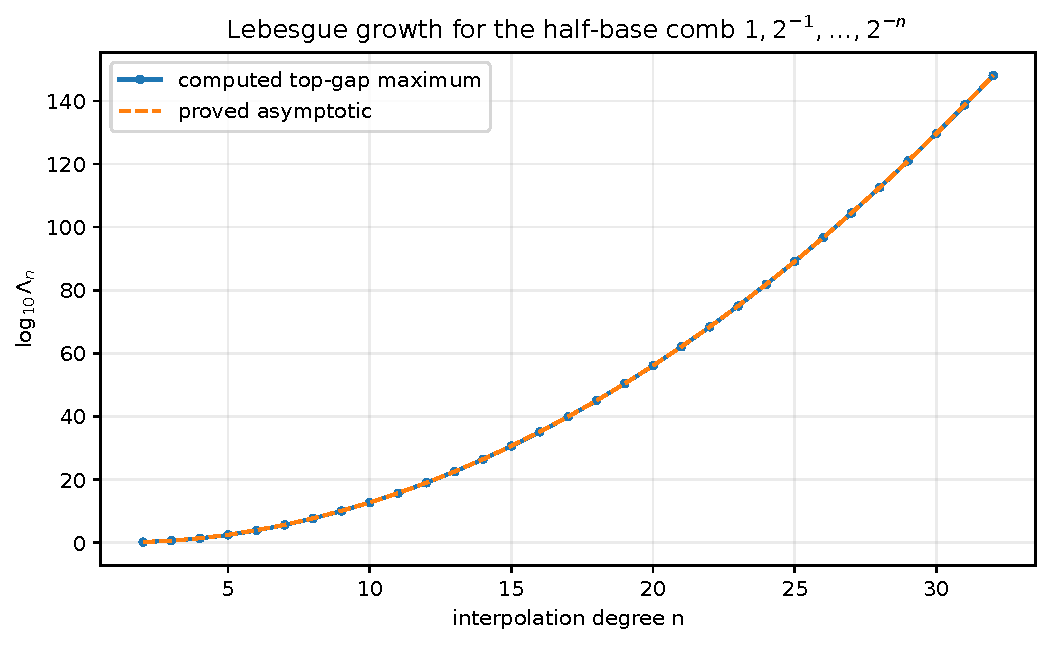
\includegraphics[width=0.90\textwidth]{lebesgue_growth.pdf}
\caption{Computed global Lebesgue maxima versus the sharp asymptotic
$2(-q;q)_\infty q^{-\binom n2}/(\EulerE n)$ for $q=1/2$.  Logarithmic arithmetic
is essential: the ordinate already exceeds $10^{148}$ at $n=32$.}
\label{fig:lebesgue-growth}
\end{figure}

\begin{figure}[p]
\centering
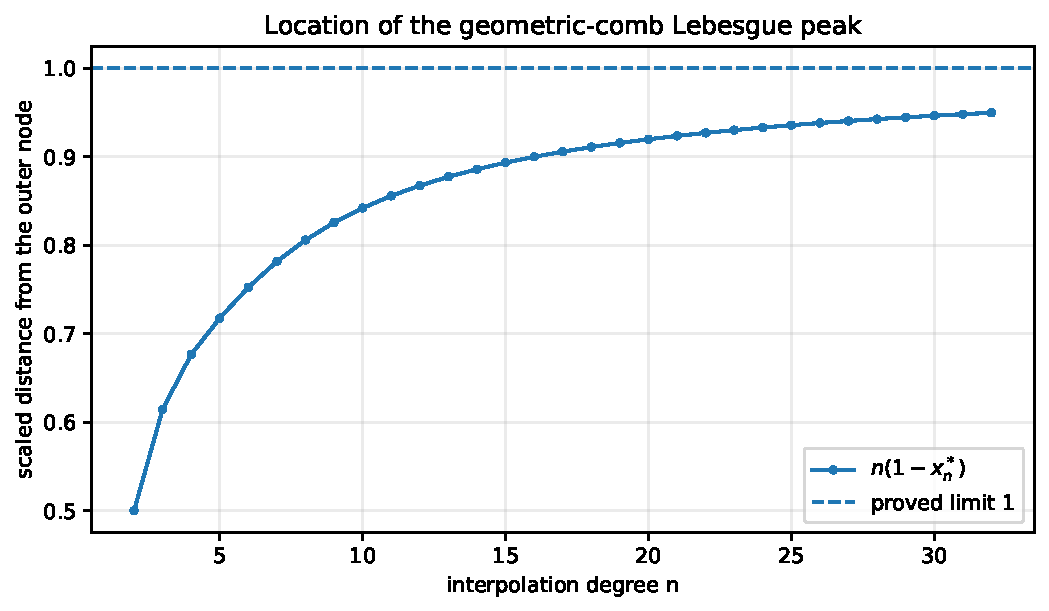
\includegraphics[width=0.90\textwidth]{lebesgue_peak_location.pdf}
\caption{The scaled boundary-layer location $n(1-x_n^*)$.  The limiting value
$1$ is the maximizer of $\alpha\EulerE^{-\alpha}$ in
\Cref{thm:lebesgue-profile}.}
\label{fig:lebesgue-peak}
\end{figure}

\section{Exact Fabius interpolation in the gap}

At $x=3/4$ the target value is exact:
\begin{equation}
 F(3/4)=1-F(1/4)=\frac{67}{72}.
 \label{eq:fabius-three-quarters}
\end{equation}
Every interpolant value in the experiment is a rational number computed
from the exact inverse-dyadic samples.  The error initially fluctuates at a
moderate scale and then enters a clear quadratic-logarithmic growth regime.

\begin{table}[htbp]
\centering
\caption{Exact Fabius interpolation diagnostics.  The third column is the
number of correct decimal digits in the extrapolated boundary value
$R_n=(\Interp_nF)(0)$, measured as $-\log_{10}|R_n|$.}
\label{tab:fabius-numerics}
\small
\begin{tabular}{@{}rrr@{}}
\toprule
$n$ & $\log_{10}|(\Interp_nF)(3/4)-67/72|$ &
$-\log_{10}|R_n|$\\
\midrule
 4 & $-0.8013$ & 2.1595\\
 8 & $ 0.8750$ & 6.7622\\
12 & $ 3.7620$ & 14.3862\\
16 & $10.5655$ & 24.8392\\
20 & $19.0624$ & 37.9904\\
24 & $29.6591$ & 53.8998\\
30 & $49.7229$ & 81.9068\\
40 & $94.5437$ & 140.6070\\
50 & $153.7151$ & 215.2423\\
\bottomrule
\end{tabular}
\end{table}

By $n=50$, the same exact interpolant that predicts $F(0)$ to more than
$215$ decimal digits is wrong at $3/4$ by about $10^{154}$.  This is a
particularly clean numerical manifestation of the stability dichotomy.

\begin{figure}[p]
\centering
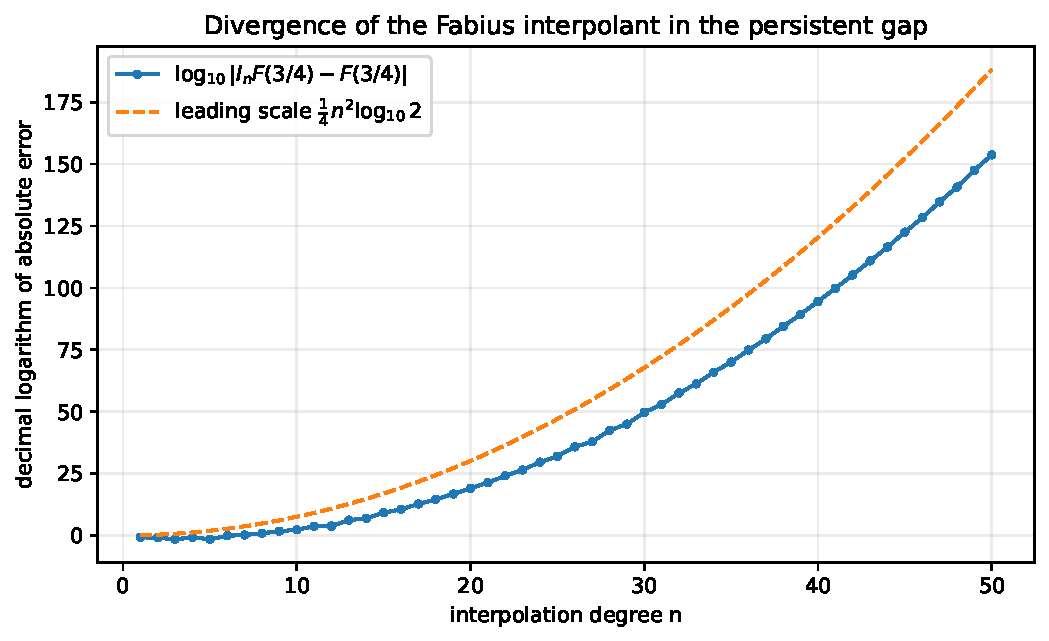
\includegraphics[width=0.90\textwidth]{fabius_gap_divergence.pdf}
\caption{Exact-rational Fabius interpolation error at $x=3/4$.  The plotted
quadratic comparison is the leading $n^2/4$ term suggested by
\Cref{conj:fabius-gap-asymptotic}; the negative $(n/2)\log n$ correction is
visible as a substantial downward displacement.}
\label{fig:fabius-gap}
\end{figure}

\begin{figure}[p]
\centering
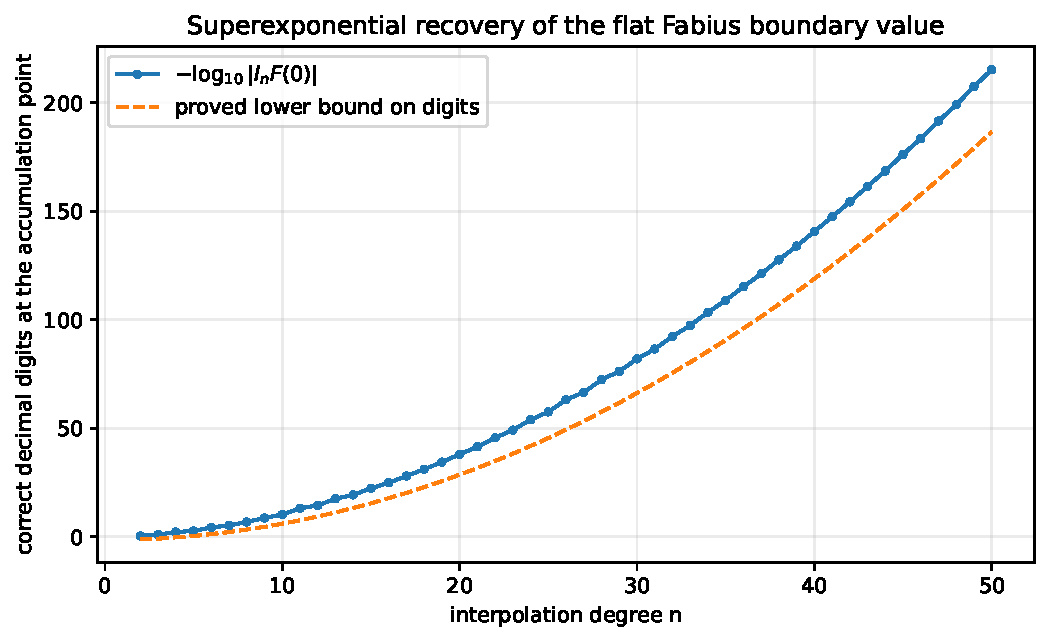
\includegraphics[width=0.90\textwidth]{fabius_boundary_residue.pdf}
\caption{Decimal digits recovered at the accumulation point.  The exact
residue is compared with the rigorous quadratic-exponential estimate from
\Cref{thm:fabius-boundary-bound}.}
\label{fig:fabius-boundary}
\end{figure}

\begin{observation}[Sign oscillation]
The gap error does not have a simple alternating sign.  Long runs of two
consecutive signs occur, reflecting the motion of a discrete saddle across
integer indices.  This supports the modulation clause in
\Cref{conj:fabius-gap-asymptotic} and argues against fitting a single smooth
prefactor from small $n$.
\end{observation}

\section{What the experiments do and do not establish}

The exact checks strongly guard against transcription errors in powers of
$q$, Gaussian reciprocity, and factorial normalizations.  The numerical
Lebesgue data confirm the proved asymptotic but are not needed for its proof.
The Fabius gap data, by contrast, are evidence for a conjecture: they show
rapid divergence at one exact rational point but do not prove the proposed
general saddle law.  The script records raw CSV data so alternative
asymptotic fits can be tested without repeating the expensive rational
interpolation.

\chapter{Further deductions, conjectures, and research directions}
\label{chap:frontiers}

This chapter separates deductions that follow mechanically from the proved
framework from genuinely open asymptotic and structural questions.

\section{Second-order Lebesgue asymptotics}

The proof of \Cref{thm:lebesgue-profile} can be expanded one order further.
The factors $(q/x;q)_{n-1}$, the ratio cloud
\eqref{eq:cardinal-ratio}, and $(1-\alpha/n)^{n-1}$ each contribute an
explicit $1/n$ correction.  This suggests the following refinement.

\begin{conjecture}[Second-order boundary layer]
\label{conj:second-order-lebesgue}
There exist explicit constants $A(q)$ and $B(q)$ such that
\begin{align}
 \frac{x_n^*}{c}
 &=1-\frac1n+\frac{A(q)}{n^2}+O_q(n^{-3}),
 \label{eq:second-order-peak-conj}\\
 \Leb_n^*
 &=\frac{2(-q;q)_\infty}{\EulerE}
   \frac{q^{-\binom n2}}{n}
   \left(1+\frac{B(q)}n+O_q(n^{-2})\right).
 \label{eq:second-order-lambda-conj}
\end{align}
The coefficients should be expressible through Lambert series such as
$\sum_{r\ge1}q^r/(1-q^r)$ and weighted Euler-cloud moments.
\end{conjecture}

A proof should follow from a uniform expansion of the ratios of the last
$O(\sqrt{\log n})$ cardinals, with the remainder controlled by the
$q^{\binom r2}$ tail.  The result would turn the qualitative convergence in
\Cref{tab:lebesgue-numerics} into a high-accuracy formula.

\section{A function-space criterion for infinite geometric Newton series}

For analytic targets, \Cref{thm:analytic-newton-convergence} supplies a
convenient sufficient condition.  A more intrinsic question starts from a
data sequence $y_j=f(cq^j)$ and asks whether the formal Newton series
\begin{equation}
 \sum_{k\ge0}
 \left(c^{-k}\sum_{j=0}^k
 \frac{(-1)^jq^{-jk+\binom{j+1}{2}}}
 {(q;q)_j(q;q)_{k-j}}y_j\right)N_k(x;c,q)
 \label{eq:formal-data-newton-series}
\end{equation}
converges in a prescribed domain.

\begin{problem}[Geometric Newton sequence spaces]
\label{prob:newton-sequence-spaces}
Characterize weighted sequence spaces $Y$ on the data $y=(y_j)$ and
coefficient spaces $G$ on the divided differences $\gamma=(\gamma_k)$ for
which the triangular Gaussian transform is an isomorphism and the Newton
synthesis map is bounded into $C(K)$, a Hardy space, or a Bergman space.
Determine the exact dependence of the norm on the location of $K$ relative
to the isolated outer node.
\end{problem}

The Richardson generating factorization
\eqref{eq:richardson-generating} indicates that Euler products provide the
correct multipliers on the data side.  A Wiener-algebra formulation may
make inversion and perturbation estimates especially transparent.

\section{Signed saddle analysis for Fabius data}

The proof of \Cref{thm:fabius-gap-upper} isolates the unsigned saddle at
\eqref{eq:fabius-saddle-location}.  To prove
\Cref{conj:fabius-gap-asymptotic}, one needs asymptotics for the signed local
packet
\begin{equation}
 \sum_{|j-j_n|\le C\sqrt{\log n}}
 (-1)^j\frac{2^{j(n-j)}a_j}{x-2^{-j}}
 \label{eq:signed-local-saddle-packet}
\end{equation}
with relative error smaller than the packet itself.

A promising route has three stages:
\begin{enumerate}
\item derive uniform saddle asymptotics for $a_j=[z^j]A(z)$ from the product
      \eqref{eq:fabius-mgf-product};
\item insert them into \eqref{eq:signed-local-saddle-packet} and apply a
      discrete Gaussian or theta transformation;
\item retain the fractional saddle displacement, which should produce a
      bounded periodic or antiperiodic modulation.
\end{enumerate}
The functional equation \eqref{eq:fabius-mgf-functional} suggests that the
moment saddle itself carries a logarithmically periodic correction.  Its
interaction with the integer Gaussian saddle may be the source of the sign
blocks seen in the experiment.

\begin{problem}[Exceptional gap points]
\label{prob:exceptional-gap-points}
Determine whether there are points $x\in(1/2,1)$ at which the leading signed
saddle cancels identically or along an infinite subsequence.  If such points
exist, classify them arithmetically and determine the next asymptotic scale.
\end{problem}

\section{Boundary-residue entire functions}

The generating function
\begin{equation}
 \mathcal R(z)=(qz;q)_\infty
 \sum_{j\ge0}\frac{q^{\binom j2}a_j}{(q;q)_j}z^j
 \label{eq:boundary-residue-entire-function}
\end{equation}
encodes all endpoint extrapolation errors.  The Euler factor has prescribed
zeros at $z=q^{-r}$, while the second factor is an entire transform of the
Fabius moments.

\begin{problem}[Zero cancellation and coefficient asymptotics]
\label{prob:boundary-entire-zeros}
Determine which Euler zeros survive in $\mathcal R$, obtain the order and
indicator of $\mathcal R$, and use its zero distribution to derive a sharp
asymptotic for $R_n$.  In particular, decide whether
\begin{equation}
 \log|R_n|=-\frac{\log2}{4}n^2+O(n\log n)
 \label{eq:boundary-residue-leading-question}
\end{equation}
has a full expansion with a parity-dependent linear term.
\end{problem}

The exact coefficient formula makes this problem accessible both to
complex-analytic saddle methods and to $2$-adic valuation experiments.

\section{Geometric Hermite stability}

The anchored factorization \eqref{eq:anchored-hermite-factorization} removes
confluent linear algebra but not operator growth.  For a flat target, its
data are rescaled by $(cq^j)^{-(m+1)}$, changing the Gaussian saddle.
A first model replaces $a_j$ by
$q^{\binom j2-j(m+1)}a_j$ in the Fabius formulas.  This predicts a movable
saddle and a phase transition when $m$ is allowed to grow with $n$.

\begin{conjecture}[Hermite saddle displacement]
\label{conj:hermite-saddle}
For $q=1/2$ and Fabius data, the dominant index in the gap for the
$m$-anchored interpolant is
\begin{equation}
 j_{n,m}=\frac n2+m+1-\frac{\log n}{2\log2}+O(1),
 \label{eq:hermite-saddle-location-conj}
\end{equation}
until it collides with the endpoint $j=n$.  The collision marks a change
from an interior Gaussian saddle to an endpoint saddle and should determine
the largest useful jet order.
\end{conjecture}

This conjecture follows from the unsigned ratio heuristic; the signed
problem may shift the practical optimum.  It can be tested by extending the
bundled exact code to \Cref{thm:anchored-hermite}.

\section{The mixed \texorpdfstring{$q$}{q}-Appell family}

The polynomials $\mathscr A_k(y;c,q)$ in
\eqref{eq:q-Appell-falling} deserve study independently of interpolation.
They combine a Sheffer/Appell deconvolution with a $q$-falling-factorial
basis.

\begin{problem}[Structure of the $q$-Appell falling powers]
\label{prob:q-Appell-structure}
Find:
\begin{enumerate}
\item raising and lowering operators for $\mathscr A_k$ involving $D_q$ and
      the ordinary derivative $D$;
\item their connection coefficients with monomials, ordinary Appell
      polynomials, and $N_k$;
\item generating functions in $k$ and continued-fraction representations;
\item zero-location and interlacing theorems for $0<q<1$;
\item asymptotics in the joint limits $k\to\infty$, $q\to1$, and
      $k(1-q)\to\tau$.
\end{enumerate}
\end{problem}

A useful starting identity is
\begin{equation}
 \sum_{k\ge0}\mathscr A_k(y;c,q)\frac{t^k}{(q;q)_k}
 =\MGF_u(D_y)^{-1}
  \sum_{k\ge0}N_k(y;c,q)\frac{t^k}{(q;q)_k},
 \label{eq:q-Appell-formal-generating}
\end{equation}
where the second series can be rewritten by the infinite $q$-binomial
theorem after normalization.  Making the operator interchange analytic is
itself a worthwhile problem.

\section{Decoder variation, total positivity, and optimal gauges}

The matrix $hB$ in \Cref{thm:gaussian-Appell-biorthogonality} is a positive
row-stochastic sampling operator.  Its right inverse $D$ has row sum one but
must use signs.  The size of its row variation controls amplification from
nodal perturbations to atom amplitudes.

\begin{problem}[Minimum-variation atomic decoder]
\label{prob:minimum-variation-decoder}
Among all right inverses of the collocation matrix $hB$, minimize a weighted
$\ell^1$ or total-variation norm subject to exact polynomial reproduction.
Compare the canonical Appell decoder with the minimizer, and determine
whether a symmetry-preserving minimizer has a closed $q$-binomial formula.
\end{problem}

The dense dictionary has an alias kernel inherited from the dyadic Fourier
zeros.  Adding an alias vector changes amplitudes without changing the
synthesized polynomial.  Convex optimization over this affine space may
substantially improve numerical conditioning while preserving every exact
identity.

\section{Stable alternatives to global gap interpolation}

The superexponential Lebesgue growth is a property of the all-node global
projector, not of geometric data in general.  Several alternatives retain
the dyadic arithmetic:
\begin{enumerate}
\item piecewise low-degree Newton or Hermite interpolation on geometric
      annuli $[cq^{j+1},cq^j]$;
\item rational barycentric interpolation with fixed local degree;
\item oversampled least squares in a logarithmic coordinate;
\item direct approximation in scaled translates of $\RvachevUp$ rather than first
      passing through one global polynomial;
\item hybrid Taylor--Newton schemes that use the flat germ near zero and a
      separate approximation across the outer gap.
\end{enumerate}
For the Fabius function, the functional equation can transport a local
approximation between adjacent dyadic scales, suggesting multiresolution
algorithms with exact consistency constraints.

\section{Complex and arithmetic geometric combs}

When $q$ is complex with $0<|q|<1$, the comb spirals into the origin.  The
algebraic formulas remain valid, while the stability problem becomes
potential-theoretic and angle-dependent.  At a root of unity the nodes
collide and ordinary interpolation becomes confluent; the denominator-free
Gaussian recurrence is then the correct algebraic replacement.

Over finite fields, the condition that $q^0,\ldots,q^n$ be distinct is
exactly an order condition in the multiplicative group.  The geometric
Vandermonde determinant in \Cref{thm:geometric-vandermonde} records its
failure cyclotomically.  This suggests a finite-field interpolation theory
whose transition matrices are literal Gaussian coefficients counting
subspaces.

\begin{problem}[Cyclotomic confluent limit]
\label{prob:cyclotomic-confluent-limit}
Develop a division-free specialization of the cardinal and residual
identities when $q$ approaches a primitive root of unity.  Identify the
resulting Hermite blocks, their cyclotomic valuations, and their relation to
$q$-Lucas congruences.
\end{problem}

\section{Formalization program}
\label{sec:formalization-program}

The theory separates into finite algebra, analytic convergence, and
asymptotics, making it well suited to staged formalization in Lean.

\begin{enumerate}
\item \textbf{Finite products.}  Define $N_k$, prove
      \eqref{eq:newton-pochhammer}, and derive the denominator product in
      \Cref{thm:geometric-barycentric} without division until the final
      field specialization.
\item \textbf{Gaussian Pascal equivalence.}  Formalize
      \Cref{thm:gaussian-pascal-basis} and its inverse as mutually inverse
      triangular matrices over a commutative ring.
\item \textbf{Residual calculus.}  Prove
      \Cref{thm:universal-moment-residual} through generating functions for
      complete homogeneous symmetric polynomials, then derive the analytic
      residual only after importing convergence lemmas.
\item \textbf{Endpoint stability.}  Formalize the exact identity
      \eqref{eq:endpoint-lebesgue} and monotone convergence of finite
      $q$-products.
\item \textbf{Boundary profile.}  Isolate the elementary limits
      $(1-\alpha/n)^n\to\EulerE^{-\alpha}$, dominated convergence for the Euler
      cloud, and the tail bound from $q^{\binom r2}$.
\item \textbf{Fabius arithmetic.}  Reuse the existing exact dyadic-value
      development to prove \Cref{thm:fabius-gaussian-transform}, the residue
      generating function, and the fixed-jet bound.
\item \textbf{Atomic synthesis.}  Formalize the finite consequence
      \eqref{eq:cardinal-up-decoder} once the repository's polynomial
      reproduction theorem for $\RvachevUp$ is available; matrix
      biorthogonality then reduces to finite sums.
\end{enumerate}

The sharp global Lebesgue theorem is the most analytically demanding new
formal target.  Its proof was deliberately organized into local profile,
away-from-boundary decay, and compactness of the scaled maximizer so these
pieces can be formalized independently.

\appendix

\chapter{Formula dictionary}
\label{app:formula-dictionary}

This appendix collects the principal transforms in one place.  It is meant
as a reference sheet rather than a substitute for the proofs.

\section{General geometric comb}

For $x_j=cq^j$, $0<q<1$, define
\[
 N_k(x)=\prod_{r=0}^{k-1}(x-cq^r),
 \qquad
 \omega_{n+1}(x)=N_{n+1}(x).
\]
Then
\begin{longtable}{@{}p{0.28\textwidth}p{0.64\textwidth}@{}}
\caption{Core geometric-comb formulas.}\label{tab:formula-dictionary-general}\\
\toprule
Object & Formula\\
\midrule
\endfirsthead
\toprule
Object & Formula\\
\midrule
\endhead
Newton/$q$-Pochhammer basis
& $N_k(x)=(-c)^kq^{\binom k2}(x/c;q^{-1})_k$\\[4pt]
Divided difference
& $[f;c,\ldots,cq^k]=D_q^kf(c)/[k]_q!$\\[4pt]
Explicit data transform
& $c^{-k}\sum_{j=0}^k
 (-1)^jq^{-jk+\binom{j+1}{2}}f(cq^j)/
 ((q;q)_j(q;q)_{k-j})$\\[6pt]
Monomial to Newton
& $x^m=\sum_{k=0}^{m}c^{m-k}\GaussianBinomial{m}{k}{q}N_k(x)$\\[4pt]
Newton to monomial
& $N_k(x)=\sum_{m=0}^{k}(-1)^{k-m}c^{k-m}
 q^{\binom{k-m}{2}}\GaussianBinomial{k}{m}{q}x^m$\\[6pt]
Barycentric weight
& $\lambda_{j,n}=c^{-n}(-1)^jq^{\binom{j+1}{2}-nj}/
 ((q;q)_j(q;q)_{n-j})$\\[6pt]
Accumulation weight
& $\mu_{j,n}=(-1)^{n-j}q^{\binom{n-j+1}{2}}/
 ((q;q)_j(q;q)_{n-j})$\\[6pt]
Endpoint Lebesgue constant
& $\Leb_n(0)=(-q;q)_n/(q;q)_n$\\[4pt]
Global Lebesgue asymptotic
& $\Leb_n^*\sim2(-q;q)_\infty q^{-\binom n2}/(\EulerE n)$\\[4pt]
Monomial residual
& $x^{n+1+r}-\Interp_nx^{n+1+r}
 =N_{n+1}(x)h_r(x,c,cq,\ldots,cq^n)$\\[6pt]
Geometric specialization
& $h_r(c,cq,\ldots,cq^n)=c^r\GaussianBinomial{n+r}{n}{q}$\\[4pt]
Jackson moment
& $\int_0^cN_k(x)\,\Differential_qx=(-1)^kc^{k+1}
 q^{\binom{k+1}{2}}/[k+1]_q$\\
\bottomrule
\end{longtable}

\section{Half-base Fabius formulas}

For $q=1/2$, $d_n=\Expectation X^n$, and $a_n=d_n/n!$,
\begin{longtable}{@{}p{0.28\textwidth}p{0.64\textwidth}@{}}
\caption{Fabius and Rvachev specialization.}\label{tab:formula-dictionary-fabius}\\
\toprule
Object & Formula\\
\midrule
\endfirsthead
\toprule
Object & Formula\\
\midrule
\endhead
Moment recurrence
& $(2^n-1)a_n=\sum_{j<n}a_j/(n-j+1)!$\\[5pt]
Rvachev half-moment
& $d_n=n\int_0^1t^{n-1}\RvachevUp(t)\,\Differential t$\\[5pt]
Inverse-dyadic value
& $F(2^{-n})=2^{-\binom n2}a_n$\\[5pt]
Newton coefficient
& $\nu_k=(q;q)_k^{-1}\sum_{j=0}^k(-1)^j
 \GaussianBinomial{k}{j}{q^{-1}}a_j$\\[6pt]
Finite interpolant
& $\Interp_nF(x)=\omega_{n+1}(x)(q;q)_n^{-1}
 \sum_{j=0}^n(-1)^j\GaussianBinomial{n}{j}{q^{-1}}a_j/(x-q^j)$\\[7pt]
Boundary residue generating function
& $\sum_{n\ge0}R_nz^n=(qz;q)_\infty
 \sum_{j\ge0}q^{\binom j2}a_jz^j/(q;q)_j$\\[7pt]
Boundary bound
& $|R_n|\le\EulerE(q;q)_\infty^{-2}q^{\Floor{n^2/4}}$\\[5pt]
Fixed-jet bound
& $|(\Interp_nF)^{(m)}(0)|\le
 \EulerE m!\binom nm(q;q)_\infty^{-2}
 q^{\Floor{n^2/4}-mn+\binom m2}$\\[7pt]
Rvachev relation
& $\RvachevUp(t)=F(1-|t|)$ and $\Interp_n\RvachevUp=1-\Interp_nF$
 on the center-directed positive comb\\
\bottomrule
\end{longtable}

\section{Atomic synthesis formulas}

For a degree bound $n$, $h=2^{-n}$ and
$K_n=\{-2^{n+1}+1,\ldots,2^{n+1}-1\}$,
\begin{align}
 \App p&=\MGF_u(D)^{-1}p
 =\sum_{r\ge0}\frac{\gamma_{2r}}{(2r)!}p^{(2r)},
 \label{eq:dictionary-App}\\
 p(x)&=h\sum_{k\in K_n}(\App p)(kh)u(x-kh),
 \qquad \deg p\le n,
 \label{eq:dictionary-synthesis}\\
 \ell_{j,n}(x)&=h\sum_{k\in K_n}
 (\App\ell_{j,n})(kh)u(x-kh),
 \label{eq:dictionary-cardinal-synthesis}\\
 (hB)D&=I_{n+1}.
 \label{eq:dictionary-right-inverse}
\end{align}

\chapter{Selected exact dyadic data}
\label{app:exact-data}

\section{Moments and inverse-dyadic values}

\begin{table}[htbp]
\centering
\caption{Regularized moments $a_n=d_n/n!$ and the corresponding values
$F(2^{-n})=2^{-\binom n2}a_n$.}
\label{tab:exact-fabius-data}
\small
\begin{tabular}{@{}rll@{}}
\toprule
$n$ & $a_n$ & $F(2^{-n})$\\
\midrule
0 & $1$ & $1$\\
1 & $1/2$ & $1/2$\\
2 & $5/36$ & $5/72$\\
3 & $1/36$ & $1/288$\\
4 & $143/32400$ & $143/2073600$\\
5 & $19/32400$ & $19/33177600$\\
6 & $1153/17146080$ & $1153/561842749440$\\
7 & $583/85730400$ & $583/179789679820800$\\
8 & $1616353/2623350240000$
  & $1616353/704200217922109440000$\\
\bottomrule
\end{tabular}
\end{table}

\section{First geometric Newton coefficients}

For
\[
 \Interp_nF(x)=\sum_{k=0}^n\nu_k
 \prod_{r=0}^{k-1}(x-2^{-r}),
\]
the exact coefficients begin
\begin{longtable}{@{}rl@{}}
\caption{First exact half-base Newton coefficients.}
\label{tab:exact-newton-coefficients}\\
\toprule
$k$ & $\nu_k$\\
\midrule
\endfirsthead
\toprule
$k$ & $\nu_k$\\
\midrule
\endhead
0 & $1$\\
1 & $1$\\
2 & $-26/27$\\
3 & $-128/27$\\
4 & $-4253248/637875$\\
5 & $189673472/19774125$\\
6 & $134859284873216/1648153544625$\\
7 & $21867230161534976/209315500167375$\\
8 & $-349286360632157831954432/204161105975753390625$\\
\bottomrule
\end{longtable}

Large numerator and denominator sizes are not numerical artifacts; they are
exact consequences of composing the Fabius moment recurrence with the
reciprocal Gaussian transform.

\chapter{Archive and reproduction notes}
\label{app:archive}

\section{Archive layout}

The delivered ZIP archive contains:
\begin{longtable}{@{}p{0.40\textwidth}p{0.52\textwidth}@{}}
\toprule
Path & Purpose\\
\midrule
\path{geometric_comb_q_fabius_report.tex}
& Complete LaTeX source of this report.\\
\path{geometric_comb_q_fabius_report.pdf}
& Rendered report.\\
\path{geometric_comb_experiments.py}
& Exact and logarithmic numerical experiments, with detailed comments.\\
\path{data/lebesgue_data.csv}
& Lebesgue endpoint values, maxima, peak locations, and asymptotic ratios.\\
\path{data/fabius_interpolation_data.csv}
& Exact-rational gap and boundary diagnostics converted to plotting fields.\\
\path{data/identity_checks.txt}
& Exact verification summary and Newton coefficients.\\
\path{figures/*.pdf}, \path{figures/*.png}
& Reproducible figures in vector and raster form.\\
\path{README.md}
& Dependencies and commands.\\
\bottomrule
\end{longtable}

\section{Commands}

From the extracted archive directory, regenerate the data and figures with
\begin{lstlisting}[language=bash]
python geometric_comb_experiments.py
\end{lstlisting}
The script requires Python 3.10 or later together with
\texttt{numpy}, \texttt{matplotlib}, and \texttt{mpmath}.  Rebuild the PDF
with a sufficiently complete TeX Live installation, for example
\begin{lstlisting}[language=bash]
pdflatex geometric_comb_q_fabius_report.tex
pdflatex geometric_comb_q_fabius_report.tex
\end{lstlisting}
Two passes resolve the table of contents and cross-references.

\section{Source boundary}

The primary source monograph and the neighboring reports were read to retain
notation and avoid duplicating already consolidated results.  The repository
snapshot used here is
\begin{equation}
 \texttt{e5175d5eb78d66f4e31db3bc506541b9bae12c57}
 \quad\text{(30 August 2026).}
 \label{eq:repository-snapshot-appendix}
\end{equation}
The sharp geometric-comb Lebesgue asymptotic, the fixed-jet Fabius estimate,
and their systematic composition with the geometric Gaussian--Appell
decoder are presented as new deductions relative to that snapshot.

\chapter{Status ledger}
\label{app:status-ledger}

\begin{longtable}{@{}p{0.47\textwidth}p{0.17\textwidth}p{0.27\textwidth}@{}}
\caption{Logical status of the principal claims.}\label{tab:status-ledger}\\
\toprule
Claim & Status & Location\\
\midrule
\endfirsthead
\toprule
Claim & Status & Location\\
\midrule
\endhead
Newton basis equals a normalized $q$-Pochhammer symbol
& proved & \Cref{chap:q-newton}\\
Iterated $D_q$ equals geometric divided difference
& proved & \Cref{thm:Dq-divided-difference}\\
Gaussian Pascal basis transform and inverse
& proved & \Cref{thm:gaussian-pascal-basis}\\
Complete-homogeneous monomial residual
& proved & \Cref{thm:monomial-residual}\\
Analytic infinite Newton convergence
& proved & \Cref{thm:analytic-newton-convergence}\\
Finite endpoint Lebesgue limit
& proved & \Cref{thm:endpoint-lebesgue}\\
Boundary-layer profile and sharp global Lebesgue constant
& proved & \Cref{thm:lebesgue-profile,thm:global-lebesgue}\\
Newton--Jackson moment formula
& proved & \Cref{thm:jackson-newton-moments}\\
Fabius half-base Gaussian transform
& proved & \Cref{thm:fabius-gaussian-transform}\\
Fabius boundary residue and fixed-jet bounds
& proved & \Cref{thm:fabius-boundary-residue,thm:fabius-fixed-jets}\\
Quadratic-logarithmic Fabius gap upper bound
& proved & \Cref{thm:fabius-gap-upper}\\
Two-sided Fabius gap asymptotic
& conjectural & \Cref{conj:fabius-gap-asymptotic}\\
Second-order Lebesgue expansion
& conjectural & \Cref{conj:second-order-lebesgue}\\
Dyadic fixed-radius polynomial synthesis by $\RvachevUp$
& proved from Fourier zero multiplicities
& \Cref{thm:up-polynomial-synthesis}\\
Gaussian--Appell cardinal decoder and right inverse
& proved & \Cref{thm:gaussian-Appell-decoder,thm:gaussian-Appell-biorthogonality}\\
Optimal growing-order geometric Hermite anchoring
& open & \Cref{prob:optimal-geometric-hermite}\\
\bottomrule
\end{longtable}

\backmatter

\begin{thebibliography}{99}

\bibitem{Andrews1986}
G.~E.~Andrews,
\newblock \emph{$q$-Series: Their Development and Application in Analysis,
Number Theory, Combinatorics, Physics, and Computer Algebra},
\newblock CBMS Regional Conference Series in Mathematics, vol.~66,
American Mathematical Society, 1986.

\bibitem{Arias2017Definition}
J.~Arias de Reyna,
\newblock An infinitely differentiable function with compact support:
definition and properties,
\newblock English translation of \emph{Revista de la Real Academia de
Ciencias Exactas, F\'isicas y Naturales de Madrid} \textbf{76} (1982),
21--38; arXiv:1702.05442, 2017.

\bibitem{Arias2018Arithmetic}
J.~Arias de Reyna,
\newblock Arithmetic of the Fabius function,
\newblock \emph{INTEGERS} \textbf{18} (2018), Article A51;
arXiv:1702.06487.

\bibitem{BerrutTrefethen2004}
J.-P.~Berrut and L.~N.~Trefethen,
\newblock Barycentric Lagrange interpolation,
\newblock \emph{SIAM Review} \textbf{46} (2004), no.~3, 501--517.

\bibitem{DLMF17}
NIST Digital Library of Mathematical Functions,
\newblock Chapter 17: $q$-hypergeometric and related functions,
\newblock F.~W.~J.~Olver et al., editors, continuously updated online.

\bibitem{Fabius1966}
J.~Fabius,
\newblock A probabilistic example of a nowhere analytic $C^\infty$-function,
\newblock \emph{Zeitschrift f\"ur Wahrscheinlichkeitstheorie und Verwandte
Gebiete} \textbf{5} (1966), 173--174.

\bibitem{GasperRahman2004}
G.~Gasper and M.~Rahman,
\newblock \emph{Basic Hypergeometric Series}, second edition,
\newblock Encyclopedia of Mathematics and its Applications, vol.~96,
Cambridge University Press, 2004.

\bibitem{Higham2004}
N.~J.~Higham,
\newblock The numerical stability of barycentric Lagrange interpolation,
\newblock \emph{IMA Journal of Numerical Analysis} \textbf{24} (2004),
no.~4, 547--556.

\bibitem{KacCheung2002}
V.~Kac and P.~Cheung,
\newblock \emph{Quantum Calculus},
\newblock Universitext, Springer, 2002.

\bibitem{Kupershmidt2000}
B.~A.~Kupershmidt,
\newblock $q$-Newton binomial: from Euler to Gauss,
\newblock \emph{Journal of Nonlinear Mathematical Physics} \textbf{7}
(2000), no.~2, 244--262; arXiv:math/0004187.

\bibitem{RvachevRvachev1972}
V.~L.~Rvachev and V.~A.~Rvachev,
\newblock On the representation of polynomials by functions with compact
support,
\newblock \emph{Mathematical Physics}, No.~11, Naukova Dumka, Kiev, 1972,
126--129.

\bibitem{StrangFix1973}
G.~Strang and G.~Fix,
\newblock A Fourier analysis of the finite element variational method,
\newblock in \emph{Constructive Aspects of Functional Analysis}, C.I.M.E.,
1973, 793--840.

\bibitem{WebbTrefethenGonnet2012}
M.~Webb, L.~N.~Trefethen, and P.~Gonnet,
\newblock Stability of barycentric interpolation formulas for extrapolation,
\newblock \emph{SIAM Journal on Scientific Computing} \textbf{34} (2012),
no.~6, A3009--A3015.

\end{thebibliography}

\end{document}
